%definira klasu dokumenta 
\documentclass[12pt]{report} 

%prostor izmedu naredbi \documentclass i \begin{document} se zove uvod. U njemu se nalaze naredbe koje se odnose na cijeli dokument

%osnovni LaTex ne može riješiti sve probleme, pa se koriste različiti paketi koji olakšavaju izradu željenog dokumenta
\usepackage[croatian]{babel} 
\usepackage{amssymb}
\usepackage{amsmath}
\usepackage{txfonts}
\usepackage{mathdots}
\usepackage{titlesec}
\usepackage{array}
\usepackage{lastpage}
\usepackage{etoolbox}
\usepackage{longtable, tabu}
\usepackage{tabularx}
\usepackage{color, colortbl}
\usepackage{adjustbox}
\usepackage{geometry}
\usepackage[classicReIm]{kpfonts}
\usepackage{hyperref}
\usepackage{fancyhdr}
\usepackage{comment}

\usepackage{float}
\usepackage{setspace}
\restylefloat{table}


\patchcmd{\chapter}{\thispagestyle{plain}}{\thispagestyle{fancy}}{}{} %redefiniranje stila stranice u paketu fancyhdr

%oblik naslova poglavlja
\titleformat{\chapter}{\normalfont\huge\bfseries}{\thechapter.}{20pt}{\Huge}
\titlespacing{\chapter}{0pt}{0pt}{40pt}


\linespread{1.3} %razmak između redaka

\geometry{a4paper, left=1in, top=1in,}  %oblik stranice

\hypersetup{ colorlinks, citecolor=black, filecolor=black, linkcolor=black,	urlcolor=black }   %izgled poveznice


%prored smanjen između redaka u nabrajanjima i popisima
\newenvironment{packed_enum}{
	\begin{enumerate}
		\setlength{\itemsep}{0pt}
		\setlength{\parskip}{0pt}
		\setlength{\parsep}{0pt}
	}{\end{enumerate}}

\newenvironment{packed_item}{
	\begin{itemize}
		\setlength{\itemsep}{0pt}
		\setlength{\parskip}{0pt}
		\setlength{\parsep}{0pt}
	}{\end{itemize}}


%boja za privatni i udaljeni kljuc u tablicama
\definecolor{LightBlue}{rgb}{0.9,0.9,1}
\definecolor{LightGreen}{rgb}{0.9,1,0.9}


%podesavanje zaglavlja i podnožja

\pagestyle{fancy}
\lhead{Programsko inženjerstvo}
\rhead{Humanitarni šetači pasa}
\lfoot{Cyfer}
\cfoot{stranica \thepage/\pageref{LastPage}}
\rfoot{\today}
\renewcommand{\headrulewidth}{0.2pt}
\renewcommand{\footrulewidth}{0.2pt}


\begin{document} 
	
	
	
	\begin{titlepage}
		\begin{center}
			\vspace*{\stretch{1.0}} %u kombinaciji s ostalim \vspace naredbama definira razmak između redaka teksta
			\LARGE Programsko inženjerstvo\\
			\large Ak. god. 2020./2021.\\
			
			\vspace*{\stretch{3.0}}
			
			\huge Humanitarni šetači pasa\\
			\Large Dokumentacija, Rev. 1\\
			
			\vspace*{\stretch{12.0}}
			\normalsize
			Grupa: \textit{Cyfer}\\
			Voditelj: \textit{Jana Juroš}\\
			
			
			\vspace*{\stretch{1.0}}
			Datum predaje: \textit{13.11.2020.}\\
	
			\vspace*{\stretch{4.0}}
			
			Nastavnik: \textit{$<$Ime i prezime nastavnika zaduženog za vašu grupu$>$}\\
		
		\end{center}

	
	\end{titlepage}

	
	\tableofcontents

	\chapter{Dnevnik promjena dokumentacije}
		
		\textbf{\textit{Kontinuirano osvježavanje}}\\
				
		
		\begin{longtabu} to \textwidth {|X[2, l]|X[13, l]|X[3, l]|X[3, l]|}
			\hline \multicolumn{1}{|l|}{\textbf{Rev.}}	& \multicolumn{1}{l|}{\textbf{Opis promjene/dodatka}} & \multicolumn{1}{|l|}{\textbf{Autori}} & \multicolumn{1}{l|}{\textbf{Datum}} \\[3pt] \hline
			\endfirsthead
			
			\hline \multicolumn{1}{|l|}{\textbf{Rev.}}	& \multicolumn{1}{l|}{\textbf{Opis promjene/dodatka}} & \multicolumn{1}{|l|}{\textbf{Autori}} & \multicolumn{1}{l|}{\textbf{Datum}} \\[3pt] \hline
			\endhead
			
			\hline 
			\endlastfoot
			
			0.1 & Napravljen predložak.	& Juroš & 22.10.2020. 		\\[3pt] \hline 
			0.2	& Napisan opis projektnog zadatka & Juroš & 27.10.2020. 	\\[3pt] \hline 
			0.3 & Dodani funkcionalni zahtjevi & Juroš & 1.11.2020 \\[3pt] \hline 
			0.3.1 & Dodan prvi dio obrazaca uporabe & Juroš & 3.11.2020 \\[3pt] \hline 
			0.3.2 & Dodan ostatak obrazaca uporabe & Bokarica, Almer, Presečki, Lukač, Sabalić, Lisica, Juroš & 4.11.2020. \\[3pt] \hline 
			0.8 & Povijest rada i trenutni status implementacije,\newline Zaključci i plan daljnjeg rada & Ivošević & 28.08.2013. \\[3pt] \hline 
			0.9 & Opisi obrazaca uporabe & Jović & 07.09.2013. \\[3pt] \hline 
			0.10 & Preveden uvod & Jović & 08.09.2013. \\[3pt] \hline 
			0.11 & Sekvencijski dijagrami & Žužak & 09.09.2013. \\[3pt] \hline 
			0.12.1 & Započeo dijagrame razreda & Horvat & 10.09.2013. \\[3pt] \hline 
			0.12.2 & Nastavak dijagrama razreda & Horvat & 11.09.2013. \\[3pt] \hline 
			\textbf{1.0} & Verzija samo s bitnim dijelovima za 1. ciklus & Ivošević & 11.09.2013. \\[3pt] \hline 
			1.1 & Uređivanje teksta -- funkcionalni i nefunkcionalni zahtjevi & Grudenić \newline Jović & 14.09.2013. \\[3pt] \hline 
			1.2 & Manje izmjene:Timer - Brojilo vremena & Grudenić & 15.09.2013. \\[3pt] \hline 
			1.3 & Popravljeni dijagrami obrazaca uporabe & Jović & 15.09.2013. \\[3pt] \hline 
			1.5 & Generalna revizija strukture dokumenta & Ivošević & 19.09.2013. \\[3pt] \hline 
			1.5.1 & Manja revizija (dijagram razmještaja) & Jović & 20.09.2013. \\[3pt] \hline 
			\textbf{2.0} & Konačni tekst predloška dokumentacije  & Ivošević & 28.09.2013. \\[3pt] \hline 
			&  &  & \\[3pt] \hline
			
			
		\end{longtabu}
	
	
		\textit{Moraju postojati glavne revizije dokumenata 1.0 i 2.0 na kraju prvog i drugog ciklusa. Između tih revizija mogu postojati manje revizije već prema tome kako se dokument bude nadopunjavao. Očekuje se da nakon svake značajnije promjene (dodatka, izmjene, uklanjanja dijelova teksta i popratnih grafičkih sadržaja) dokumenta se to zabilježi kao revizija. Npr., revizije unutar prvog ciklusa će imati oznake 0.1, 0.2, …, 0.9, 0.10, 0.11.. sve do konačne revizije prvog ciklusa 1.0. U drugom ciklusu se nastavlja s revizijama 1.1, 1.2, itd.}
	\chapter{Opis projektnog zadatka}
		
		\section{Motivacija i cilj}
		Cilj ovog projekta je stvoriti aplikaciju koja može na jednostavan i brz način spojiti građane i udruge za životinje kako bi se organizirale šetnje nezbrinutih pasa.\\
		Naime, broj nezbrinutih životinja raste u Hrvatskoj te je procijenjeno da ima 10 000 napuštenih životinja. Skloništa i udruge za nezbrinute životinje spašavaju ranjene i
		nezbrinute životinje, te žele potaknuti građane na angažiranost, pomoć pri brizi za
		životinje i za njihove udomljavanje. Šetnja je psima primarna potreba, a skloništa nemaju dovoljno resursa za hranu, a kamoli za plaćanje šetnji. Pretpostavljamo da bi se ljudi rado uključili u šetanje pasa kad bi postojao način, pogotovo ako planiraju usvojiti jednoga. Naša aplikacija im to odsad može i omogućiti.\\
		
		\section{Postojeća slična rješenja}
		Što se tiče postojećih rješenja iste tematike, ne postoji previše sličnosti s našim projektom. Postoje 3 web-stranice koje mogu spojiti šetače s vlasnicima pasa, no vlasnici plaćaju za te usluge te udruge nisu uključene. Prve dvije funkcioniraju na temelju oglasa - korisnik stavi oglas sa slikom svog kućnog ljubimca, vrijeme kad mu je potrebna usluga te koliko će platiti. Te stranice su:
		\begin{description}
		\item [Njuškalo:] -- najveći online oglasnik u Hrvatskoj  
		\item [Čuvalica:] -- Nacionalni portal za brigu o obitelji -- briga za djecu, starije, ljubimce 
		\end{description}
		
		Također, postoji web-stranica obrta \textbf{PETS STEP} koji nudi uslugu čuvanja i šetnje pasa. Na stranici imaju kontakt i cjenik.\par
		Kao što možemo vidjeti, u Hrvatskoj ne postoji usluga slična našoj, no u svijetu ih možemo pronaći. Najsličniji primjer bi bila web platforma \textbf{Walkzee} -- \textit{``1st free online platform connecting shelter dogs in need of a walk to dog lovers looking for a walking buddy!´´} Walkzee su stvorili Cristina i Charlie Saunders 2015. te je ideja identična kao ideja iza našeg projekta. Nažalost, njihova stranica nije zaživjela te nema mnogo udruga niti pasa na stranici. Naime, ima samo 10 stranica te 14 pasa. Osim toga, stranica izgleda nedovršeno pa ne znamo je li ikada uopće funkcionirala. Nadamo se da njihov neuspjeh leži u lošoj egzekuciji, a ne u lošoj ideji odnosno indiferentnosti javnosti prema napuštenim životinjama. 
		
		\begin{figure}[htb]
			\centering
			
\includegraphics[scale=0.3]{slike/walkzee.png}
			\caption{Walkzee -- naslovna stranica}
			\label{fig:walkzee}
		\end{figure}

		
		\begin{figure}[htb]
			\centering
			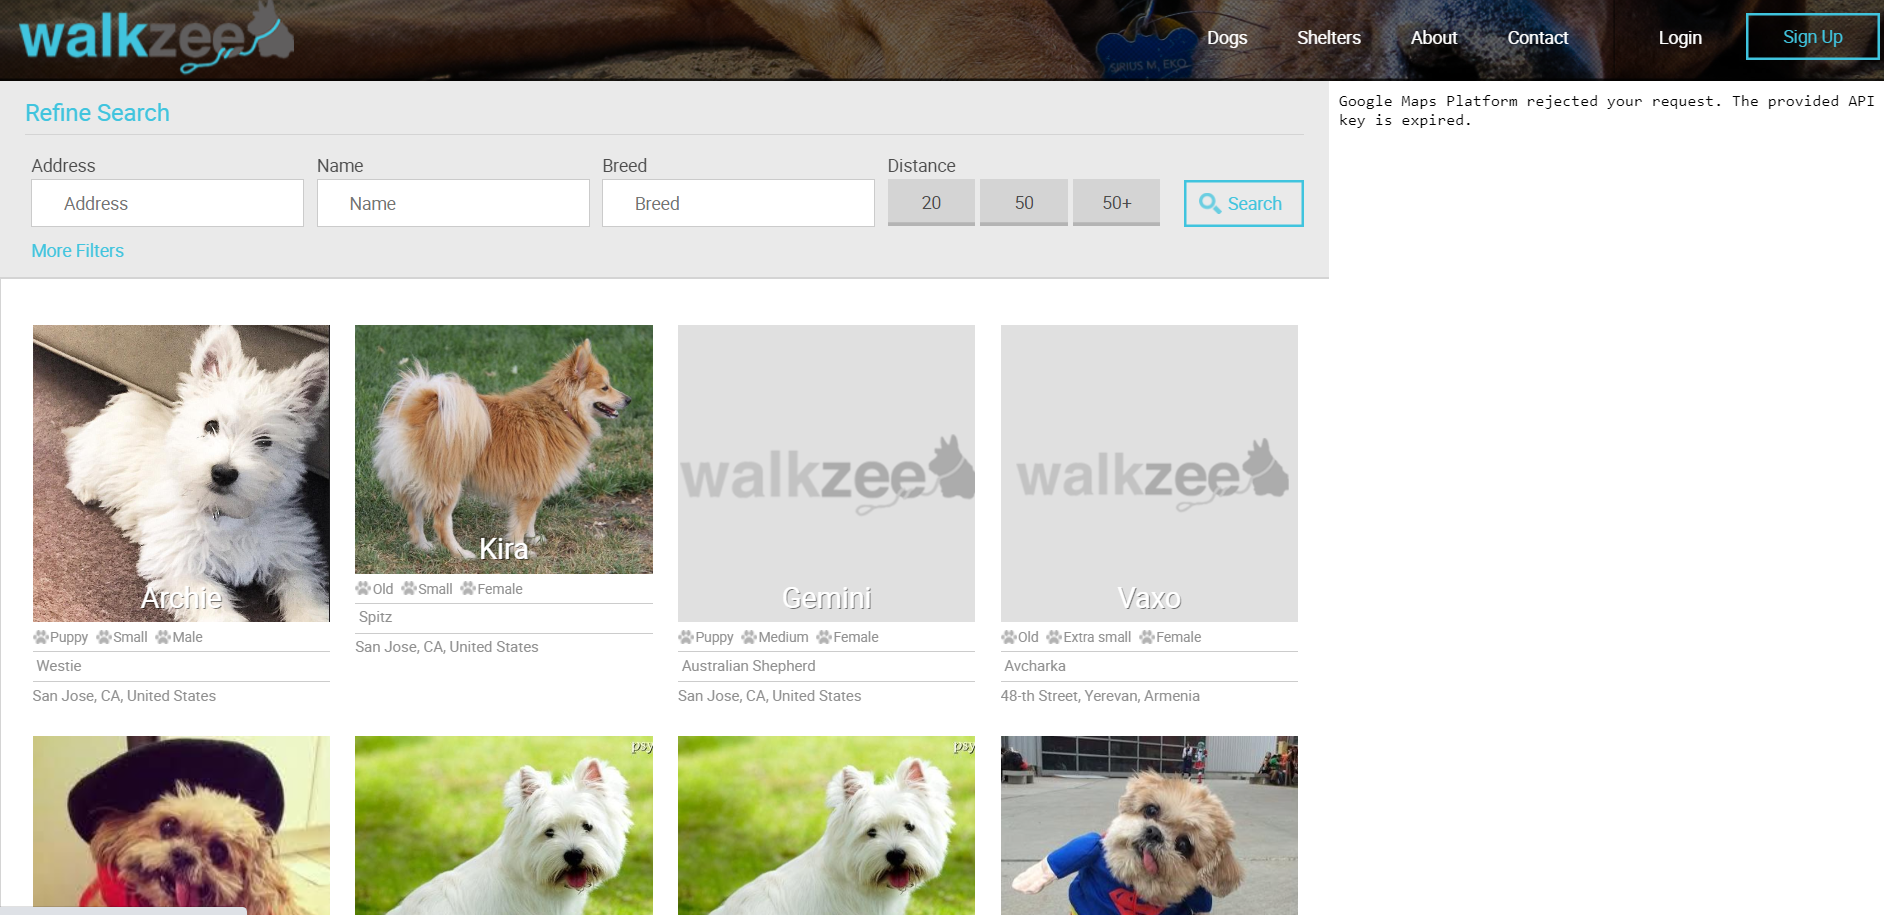
\includegraphics[scale=0.3]{slike/walkzeeDogs.png}
			\caption{Walkzee -- pregled pasa}
			\label{fig:walkzee}
		\end{figure}
	
	\section{Opseg projektnog zadatka}
	  \vspace{15pt}
		Glavni zadatak aplikacije je povezati udruge za životinje s građanima koji imaju
	želju i vrijeme za šetanje pasa, te time povećati izglede udomljavanja pasa i psihološkog
	efekta dobrobiti socijalizacije za psa i za čovjeka. \par \vspace{10pt}
	Aplikaciju će koristiti registrirane udruge za životinje, registrirani
	građani i javni posjetitelji koji nisu registrirani i imaju mogućnost
	pristupa naslovnoj stranici aplikacije i detaljima profila udruge.
	Udruge i građani se mogu registrirati, pri čemu građani upisuju sljedeće podatke:
	\begin{itemize}
		\item ime
		\item prezime
		\item korisničko ime
		\item adresa e-pošte
	\end{itemize} 
	a udruge još dodatno:
	\begin{itemize}
		\item naziv udruge
		\item OIB udruge
	\end{itemize}
	 \vspace{10pt}
	\underline{Javni posjetitelj} može doći u aplikaciju i
	pregledati sve udruge na naslovnoj stranici, zatim otići na detalje profila pojedine udruge,
	a osim toga ima i uvid u rang listu registriranih šetača.  Rang lista prikazuje poredak šetača
	s obzirom na broj šetnji, broj pasa, te duljinu šetnje koju su odradili u prethodnih mjesec
	dana.
	Na profilu pojedine udruge, posjetitelj može dobiti uvid u profile pasa,
	statistike o šetanjima svih pasa, lokaciju, te mogućnost prijave za šetanje pasa (ako se registrira). Statistika
	o šetnjama pruža informacije koji psi su češće bili u šetnji od ostalih, te time koji psi imaju
	veću potrebu za šetnjom.
	Ukoliko posjetitelj odluči pripomoći udruzi i priključiti se šetnji
	pasa, ima opciju registracije. Registracijom posjetitelj postaje registrirani građanin. 
	
	
	  \vspace{15pt} \par 
	  
	  	\underline{Registrirani građanin} ima opciju prijave u vlastiti profil i pregleda vlastitih rasporeda šetanja,
	  vlastitih statistika šetnji, zajedno s mogućnošću označavanja statistike šetanja kao javnih;
	  kako bi podaci građana dospjeli na rang listu na javnoj stranici.
	  Svi registrirani korisnici imaju mogućnost mijenjanja podataka u svom profilu.
	   Građanin može odabrati psa/e, odabrati željeni
	  termin šetnje i prijaviti se za šetača. Termin šetnje se odabire u obliku datuma i vremena.
	  Nakon uspješnog „rezerviranja“ psa za šetnju, termin za odabranog psa vidljiv je na
	  kalendaru registriranim građanima. Građani imaju opciju skinuti 
	  raspored za odabrani dan, tjedan ili mjesec u PDF obliku.\par
	  \vspace{15pt}
	
	Svaka \underline{registrirana udruga} može kreirati vlastiti profil koji će se prikazivati na javnoj
	stranici. Stranica udruge će sadržavati neke bitne detalje vezanu uz samu udrugu poput: 
	\begin{itemize}
		\item ime udruge
		\item voditelj udruge
		\item lokacija udruge
		\item kontakt: e-mail adresa
		\item OIB udruge
		\item IBAN udruge (za moguće donacije)
	\end{itemize}
Također, svaka udruga održava listu vlastitih pasa koji su raspoloživi za šetnju. Neke od bitnih informacija o pojedinom psu uključuju: 
	\begin{itemize}
		\item ime psa
		\item vrsta psa (ako je poznata)
		\item slika psa 
		\item opis psa (osobnost, izgled)
		\item dob psa
		\item raspored odnosno raspoloživost psa za određeni vremenski period (datum i vrijeme) 
		\item za kakve šetnje je pas predodređen (skupne ili individualne šetnje). 
	\end{itemize}
Svaka udruga ima opciju mijenjati svoj profil. To može uključivati mijenjanje vlastitih podataka (vezanih uz samu udrugu) te uređivanje liste i profila pasa. 




	  

		\iffalse
		\section{Primjeri u \LaTeX u}
		
		\textit{Ovo potpoglavlje izbrisati.}\\

		U nastavku se nalaze različiti primjeri kako koristiti osnovne funkcionalnosti \LaTeX a koje su potrebne za izradu dokumentacije. Za dodatnu pomoć obratiti se asistentu na projektu ili potražiti upute na sljedećim web sjedištima:
		\begin{itemize}
			\item Upute za izradu diplomskog rada u \LaTeX u - \url{https://www.fer.unizg.hr/_download/repository/LaTeX-upute.pdf}
			\item \LaTeX\ projekt - \url{https://www.latex-project.org/help/}
			\item StackExchange za Tex - \url{https://tex.stackexchange.com/}\\
		
		\end{itemize} 	


		
		\noindent \underbar{podcrtani tekst}, \textbf{podebljani tekst}, 	\textit{nagnuti tekst}\\
		\noindent \normalsize primjer \large primjer \Large primjer \LARGE {primjer} \huge {primjer} \Huge primjer \normalsize
				
		\begin{packed_item}
			
			\item  primjer
			\item  primjer
			\item  primjer
			\item[] \begin{packed_enum}
				\item primjer
				\item[] \begin{packed_enum}
					\item[1.a] primjer
					\item[b] primjer
				\end{packed_enum}
				\item primjer
			\end{packed_enum}
			
		\end{packed_item}
		
		\noindent primjer url-a: \url{https://www.fer.unizg.hr/predmet/proinz/projekt}
		
		\noindent posebni znakovi: \# \$ \% \& \{ \} \_ 
		$|$ $<$ $>$ 
		\^{} 
		\~{} 
		$\backslash$ 
		
		\begin{longtabu} to \textwidth {|X[8, l]|X[8, l]|X[16, l]|} %definicija širine tablice, širine stupaca i poravnanje
			
			%definicija naslova tablice
			\hline \multicolumn{3}{|c|}{\textbf{naslov unutar tablice}}	 \\[3pt] \hline
			\endfirsthead
			
			%definicija naslova tablice prilikom prijeloma
			\hline \multicolumn{3}{|c|}{\textbf{naslov unutar tablice}}	 \\[3pt] \hline
			\endhead
			
			\hline 
			\endlastfoot
			
			\rowcolor{LightGreen}IDKorisnik & INT	&  	Lorem ipsum dolor sit amet, consectetur adipiscing elit, sed do eiusmod  	\\ \hline
			korisnickoIme	& VARCHAR &   	\\ \hline 
			email & VARCHAR &   \\ \hline 
			ime & VARCHAR	&  		\\ \hline 
			\cellcolor{LightBlue} primjer	& VARCHAR &   	\\ \hline 
			
		\end{longtabu}
		

		\begin{table}[H]
			
			\begin{longtabu} to \textwidth {|X[8, l]|X[8, l]|X[16, l]|} 
				
				\hline 
				\endfirsthead
				
				\hline 
				\endhead
				
				\hline 
				\endlastfoot
				
				\rowcolor{LightGreen}IDKorisnik & INT	&  	Lorem ipsum dolor sit amet, consectetur adipiscing elit, sed do eiusmod  	\\ \hline
				korisnickoIme	& VARCHAR &   	\\ \hline 
				email & VARCHAR &   \\ \hline 
				ime & VARCHAR	&  		\\ \hline 
				\cellcolor{LightBlue} primjer	& VARCHAR &   	\\ \hline 
				
				
			\end{longtabu}
	
			\caption{\label{tab:referencatablica} Naslov ispod tablice.}
		\end{table}
		
		
		%unos slike
		\begin{figure}[H]
			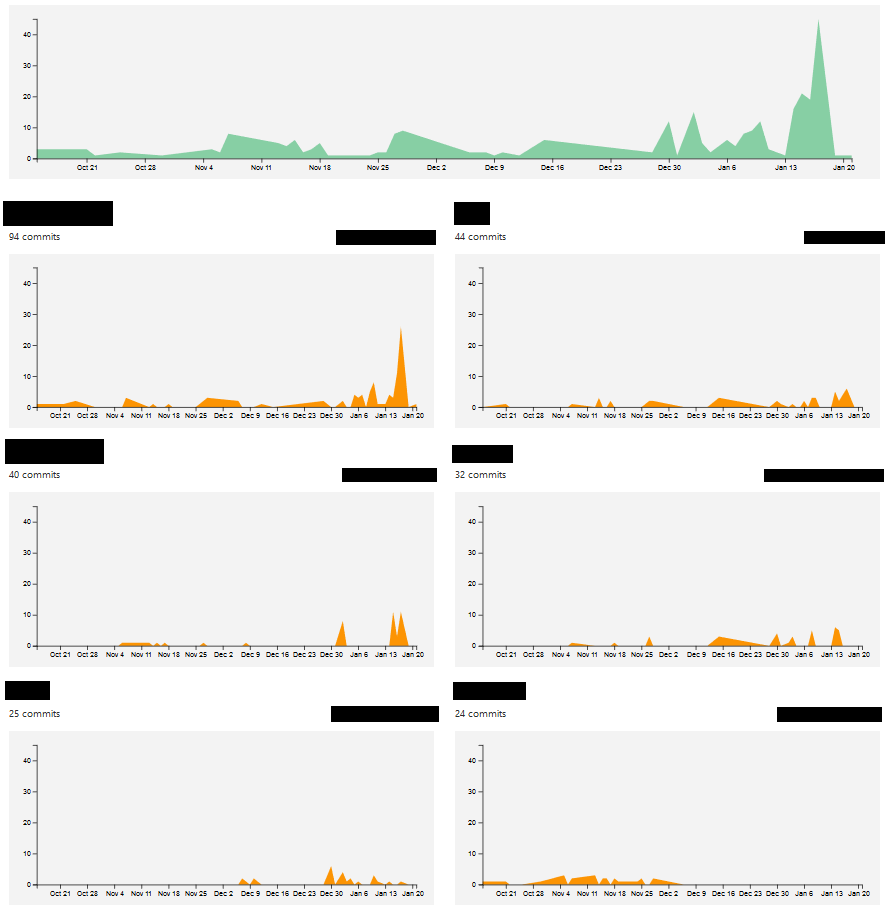
\includegraphics[scale=0.4]{slike/aktivnost.PNG} %veličina slike u odnosu na originalnu datoteku i pozicija slike
			\centering
			\caption{Primjer slike s potpisom}
			\label{fig:promjene}
		\end{figure}
		
		\begin{figure}[H]
			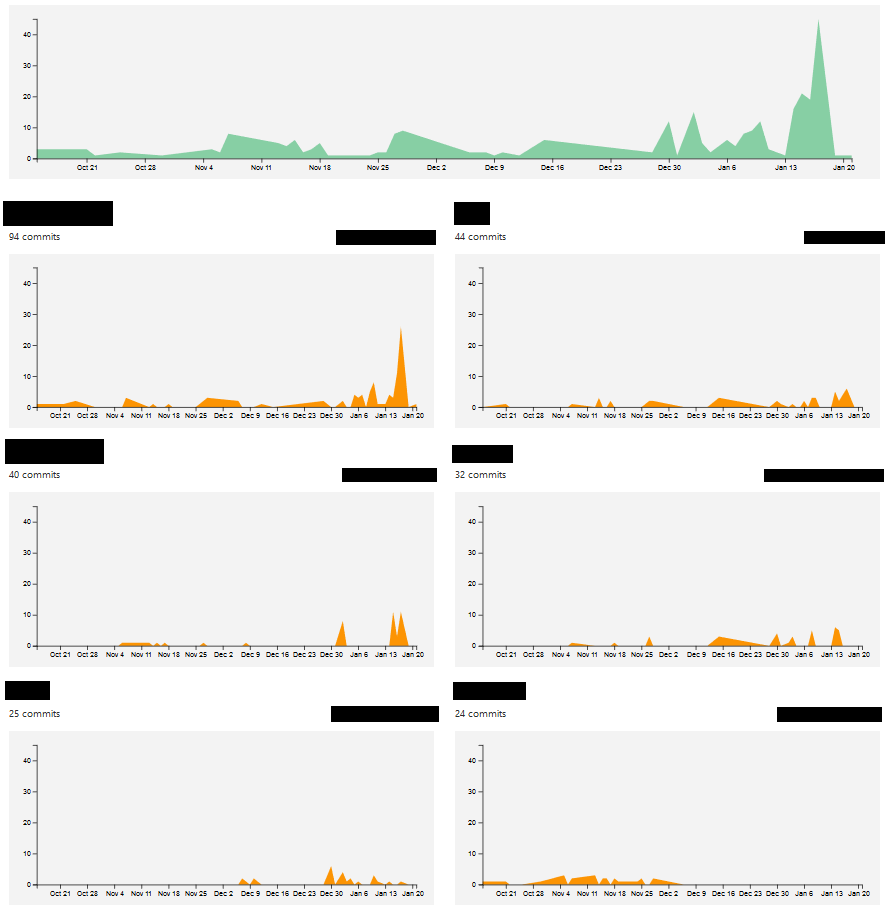
\includegraphics[width=.9\linewidth]{slike/aktivnost.PNG} %veličina u odnosu na širinu linije
			\caption{Primjer slike s potpisom 2}
			\label{fig:promjene2} %label mora biti drugaciji za svaku sliku
		\end{figure}
		
		Referenciranje slike \ref{fig:promjene2} u tekstu.
		
		
		\fi
		\eject
		
	
	\chapter{Specifikacija programske potpore}
		
	\section{Funkcionalni zahtjevi}
			
			\textbf{\textit{dio 1. revizije}}\\
			
			\textit{Navesti \textbf{dionike} koji imaju \textbf{interes u ovom sustavu} ili  \textbf{su nositelji odgovornosti}. To su prije svega korisnici, ali i administratori sustava, naručitelji, razvojni tim.}\\
				
			\textit{Navesti \textbf{aktore} koji izravno \textbf{koriste} ili \textbf{komuniciraju sa sustavom}. Oni mogu imati inicijatorsku ulogu, tj. započinju određene procese u sustavu ili samo sudioničku ulogu, tj. obavljaju određeni posao. Za svakog aktora navesti funkcionalne zahtjeve koji se na njega odnose.}\\
			
			
			\noindent \textbf{Dionici:}
			
			\begin{packed_enum}
				
				\item Voditelji udruga
				\item Šetači pasa (registrirani korisnici)			
				\item Zaposlenici i volonteri u udrugama
				\item Administrator
				\item Razvojni tim
				
			\end{packed_enum}
			\vspace{5mm}
			
			\noindent \textbf{Aktori i njihovi funkcionalni zahtjevi:}
			
			
			\begin{packed_enum}
				\item  \underbar{Javni posjetitelj (inicijator) može:}
				
				\begin{packed_enum}
					
					\item pregledati listu udruga na naslovnoj stranici
					\item odabrati udrugu te pregledati: 
					\begin{packed_enum}
						
						\item  detalje profila udruge:
						\begin{packed_enum}
							\item ime udruge
							\item voditelj udruge
							\item kontakt: email adresa i broj mobitela
							\item lokacija
							\item OIB udruge
							\item IBAN udruge - u slučaju da netko želi napraviti donaciju
						\end{packed_enum}
						\item  listu pasa iz te udruge koji su raspoloživi za šetnju
					\end{packed_enum}
				
					\item odabrati profil psa iz liste pasa te pregledati detalje profila psa: 
					\begin{packed_enum}
						\item ime psa
						\item vrsta psa (ako je poznata)
						\item slika psa
						\item opis psa (osobnost, izgled)
						\item dob psa
						\item raspored odnosno raspoloživost psa za određeni vremenski period (datum i vrijeme) 
						\item vrsta šetnje za koju je pas predodređen (skupna ili individualna)
					\end{packed_enum} 
					\item otvoriti statistiku svih pasa raspoloživih za šetnju i vidjeti koji pas se najmanje šteao, odnosno kojem psu je šetnja najpotrebnija
					\item registrirati se u sustav kao građanin - za stvaranje korisničkog računa potrebni su mu:
					\begin{packed_enum}
						\item ime i prezime
						\item e-mail adresa
						\item lozinka 
					\end{packed_enum}
					\item registrirati u sustav svoju udrugu - za stvaranje korisničkog računa potrebni su mu:
					\begin{packed_enum}
						\item ime i prezime
						\item e-mail adresa
						\item lozinka 
						\item naziv udruge
						\item OIB udruge
					\end{packed_enum}
					\item  otvoriti rang-listu svih registriranih šetača poredanu s obzirom na broj šetnji, broj pasa te duljinu šetnje koju su odradili u proteklih mjesec dana
					
				\end{packed_enum}
				\vspace{5mm}
			
				\item  \underbar{Prijavljeni građanin (inicijator)} preuzima sve funkcionalnosti javnog posjetitelja te može dodatno:
				\begin{packed_enum}
					\item prijaviti se u sutav (s e-mailom i lozinkom)
					\item uređivati vlastiti profil
					\item obrisati vlastiti profil
					\item odabrati psa te na njegovom profilu prijaviti se za šetnju
					\item pregledati vlastiti raspored šetnji te skinuti (eng. download) raspored za odabrani dan, tjedan ili mjesec, u PDF obliku
					\item pregledati vlastitu statistiku šetanja
					\item označiti vlastite statistike šetanja kao \underbar{javne} kako bi podaci građana dospjeli na rang listu na javnoj stranici
				\end{packed_enum}
				\vspace{5mm}
			
				\item  \underbar{Prijavljena udruga (inicijator)} preuzima sve funkcionalnosti javnog posjetitelja te može dodatno:
				\begin{packed_enum}
					\item prijaviti se u sutav (s e-mailom i lozinkom)
					\item uređivati vlastiti profil
					\item dodavati i brisati pse iz liste raspoloživih pasa te udruge
					\item uređivati profile pasa koji su iz te udruge 
					\item obrisati vlasitti profil
				\end{packed_enum}
				\vspace{5mm}
			
				\item  \underbar{Administrator(inicijator)} može:
				\begin{packed_enum}
					\item vidjeti popis svih registriranih korisnika i udruga njihovih osobnih podataka
					\item dodati ili obrisati udruge
					\item ???
				\end{packed_enum}
				\vspace{5mm}
			
				\item  \underbar{Baza podataka (sudionik)}:
				\begin{packed_enum}
					\item pohranjuje sve podatke o korisnicima i udrugama 
					\item ???
				\end{packed_enum}
			
			\end{packed_enum}
			
			\eject 
			
			
				
			\subsection{Obrasci uporabe}
				
				\textbf{\textit{dio 1. revizije}}
				
				\subsubsection{Opis obrazaca uporabe}
					\textit{Funkcionalne zahtjeve razraditi u obliku obrazaca uporabe. Svaki obrazac je potrebno razraditi prema donjem predlošku. Ukoliko u nekom koraku može doći do odstupanja, potrebno je to odstupanje opisati i po mogućnosti ponuditi rješenje kojim bi se tijek obrasca vratio na osnovni tijek.}\\
					

					\noindent \underbar{\textbf{UC$<$broj obrasca$>$ -$<$ime obrasca$>$}}
					\begin{packed_item}
	
						\item \textbf{Glavni sudionik: }$<$sudionik$>$
						\item  \textbf{Cilj:} $<$cilj$>$
						\item  \textbf{Sudionici:} $<$sudionici$>$
						\item  \textbf{Preduvjet:} $<$preduvjet$>$
						\item  \textbf{Opis osnovnog tijeka:}
						
						\item[] \begin{packed_enum}
	
							\item $<$opis korak jedan$>$
							\item $<$opis korak dva$>$
							\item $<$opis korak tri$>$
							\item $<$opis korak četiri$>$
							\item $<$opis korak pet$>$
						\end{packed_enum}
						
						\item  \textbf{Opis mogućih odstupanja:}
						
						\item[] \begin{packed_item}
	
							\item[2.a] $<$opis mogućeg scenarija odstupanja u koraku 2$>$
							\item[] \begin{packed_enum}
								
								\item $<$opis rješenja mogućeg scenarija korak 1$>$
								\item $<$opis rješenja mogućeg scenarija korak 2$>$
								
							\end{packed_enum}
							\item[2.b] $<$opis mogućeg scenarija odstupanja u koraku 2$>$
							\item[3.a] $<$opis mogućeg scenarija odstupanja  u koraku 3$>$
							
						\end{packed_item}
					\end{packed_item}
				
				\noindent \underbar{\textbf{UC1 - Pregled profila udruga i pasa}}
				\begin{packed_item}
					
					\item \textbf{Glavni sudionik:} javni posjetitelj
					\item  \textbf{Cilj:} Otvoriti profil pojedine udruge ili psa
					\item  \textbf{Sudionici:} Baza podataka
					\item  \textbf{Preduvjet:} -
					\item  \textbf{Opis osnovnog tijeka:}
					
					\item[] \begin{packed_enum}
						
						\item Korisnik sa naslovne strane odabire udrugu koju želi proučiti
						\item Iz liste pasa te udruge korisnik odabire psa koji ga zanima
						\item Korisnik može proučavati podatke i raspored željenog psa
					\end{packed_enum}
					
					\item  \textbf{Opis mogućih odstupanja:}
					
					\item[] \begin{packed_item}
						
						\item [2.a] Odabir već zauzete email adrese, unos podataka u neispravnom formatu
						\item[] \begin{packed_enum}
							
							\item Sustav obavjestava korisnika o neuspjelom upisu i vraća ga na stranicu za registraciju
							\item Korisnik mijenja potrebne podatke te zavrsava unos ili odustaje od registracije
							
						\end{packed_enum}
					\end{packed_item}
				\end{packed_item}
			
			
	
		
				\noindent \underbar{\textbf{UC3 - Registracija građanina ili udruge u sustav}}
				\begin{packed_item}
					
					\item \textbf{Glavni sudionik:} javni posjetitelj
					\item  \textbf{Cilj:} Stvoriti korisnički račun za pristup sustavu
					\item  \textbf{Sudionici:} Baza podataka
					\item  \textbf{Preduvjet:} -
					\item  \textbf{Opis osnovnog tijeka:}
					
					\item[] \begin{packed_enum}
						
						\item Korisnik odabire opciju (gumb) za registraciju
						\item Korisnik unosi potrebne korisničke podatke (ime, prezime, email adresa i lozinka za građanina te dodatno ime udruge i OIB udruge za udrugu)
						\item Korisnik prima obavijest o uspješnoj registraciji
					\end{packed_enum}
					
					\item  \textbf{Opis mogućih odstupanja:}
					
					\item[] \begin{packed_item}
						
						\item [2.a] Odabir već zauzete email adrese, unos podataka u neispravnom formatu
						\item[] \begin{packed_enum}
							
							\item Sustav obavjestava korisnika o neuspjelom upisu i vraća ga na stranicu za registraciju
							\item Korisnik mijenja potrebne podatke te zavrsava unos ili odustaje od registracije

						\end{packed_enum}
					\end{packed_item}
				\end{packed_item}
			
				\noindent \underbar{\textbf{UC4 - Prijava građanina ili udruge u sustav}}
				\begin{packed_item}
					
					\item \textbf{Glavni sudionik:} registrirani građanin/registrirana udruga
					\item  \textbf{Cilj:} Dobiti pristup odgovarajućem korisničkom sučelju
					\item  \textbf{Sudionici:} Baza podataka
					\item  \textbf{Preduvjet:} Registracija građanina ili udruge u sustav
					\item  \textbf{Opis osnovnog tijeka:}
					
					\item[] \begin{packed_enum}
						
						\item Unos email adrese i lozinke
						\item Potvrda o ispravnosti unesenih podataka
						\item Pristup odgovarajućim korisničkim funkcijama (ovisi prijavljuje li se građanin ili udruga)
					\end{packed_enum}
					
					\item  \textbf{Opis mogućih odstupanja:}
					
					\item[] \begin{packed_item}
						
						\item [2.a] Neispravno ime/lozinka
						\item[] \begin{packed_enum}
							
							\item Sustav obavještava korisnika o neuspjelom upisu i vraća ga na stranicu za prijavu
							
						\end{packed_enum}
					\end{packed_item}
				\end{packed_item}
				
		
				                                                                 
				
					
				\subsubsection{Dijagrami obrazaca uporabe}
					
					\textit{Prikazati odnos aktora i obrazaca uporabe odgovarajućim UML dijagramom. Nije nužno nacrtati sve na jednom dijagramu. Modelirati po razinama apstrakcije i skupovima srodnih funkcionalnosti.}
				\eject		
				
			\subsection{Sekvencijski dijagrami}
				
				\textbf{\textit{dio 1. revizije}}\\
				
				\textit{Nacrtati sekvencijske dijagrame koji modeliraju najvažnije dijelove sustava (max. 4 dijagrama). Ukoliko postoji nedoumica oko odabira, razjasniti s asistentom. Uz svaki dijagram napisati detaljni opis dijagrama.}
				\eject
	
		\section{Ostali zahtjevi}
		
			\textbf{\textit{dio 1. revizije}}\\
		 
			 \textit{Nefunkcionalni zahtjevi i zahtjevi domene primjene dopunjuju funkcionalne zahtjeve. Oni opisuju \textbf{kako se sustav treba ponašati} i koja \textbf{ograničenja} treba poštivati (performanse, korisničko iskustvo, pouzdanost, standardi kvalitete, sigurnost...). Primjeri takvih zahtjeva u Vašem projektu mogu biti: podržani jezici korisničkog sučelja, vrijeme odziva, najveći mogući podržani broj korisnika, podržane web/mobilne platforme, razina zaštite (protokoli komunikacije, kriptiranje...)... Svaki takav zahtjev potrebno je navesti u jednoj ili dvije rečenice.}
			 
			 
			 
	
	\chapter{Arhitektura i dizajn sustava}
		
		\iffalse
		\textbf{\textit{dio 1. revizije}}\\

		\textit{ Potrebno je opisati stil arhitekture te identificirati: podsustave, preslikavanje na radnu platformu, spremišta podataka, mrežne protokole, globalni upravljački tok i sklopovsko-programske zahtjeve. Po točkama razraditi i popratiti odgovarajućim skicama:}
	\begin{itemize}
		\item 	\textit{izbor arhitekture temeljem principa oblikovanja pokazanih na predavanjima (objasniti zašto ste baš odabrali takvu arhitekturu)}
		\item 	\textit{organizaciju sustava s najviše razine apstrakcije (npr. klijent-poslužitelj, baza podataka, datotečni sustav, grafičko sučelje)}
		\item 	\textit{organizaciju aplikacije (npr. slojevi frontend i backend, MVC arhitektura) }		
	\end{itemize}
\fi
	S najviše razine apstrakcije, arhitekturu možemo podijeliti na tri podsustava:
	\begin{itemize}
		\item Web poslužitelj
		\item Web aplikacija
		\item Baza podataka
	\end{itemize}

\vspace{15pt} 
\begin{figure}[H]
	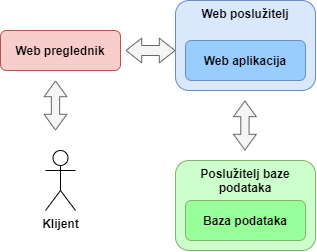
\includegraphics[scale=0.75]{slike/apstraktna-arh.PNG} %veličina slike u odnosu na originalnu datoteku i pozicija slike
	\centering
	\caption{Apstraktna arhitektura sustava}
	\label{fig:arh}
\end{figure}
\vspace{15pt}

\underline{Web preglednik} (eng. web browser) je program koji korisniku omogućuje pregled web-stranica i multimedijalnih sadržaja vezanih uz njih. Preglednik omogućuje komunikaciju između klijenta i poslužitelja. Dakle, korisnik će putem preglednika slati zahtjeve poslužitelju te će preglednik znati prikazati sadržaj koji poslužitelj vraća. \par
\vspace{10pt}
\underline{Web poslužitelj}  ima zadatak da pohranjuje, obrađuje i dostavlja klijentima web
stranice. Komunikacija između web poslužitelja i web klijenta (najčešće, web
pretraživača) odvija se korištenjem HTTP i drugih sličnih protokola (HTTPS,
HTTP/2 i različitih nadogradnji tih protokola). U komunikaciji putem HTTP-a, web
poslužitelj tipično sluša nadolazeće zahtjeve klijenata na portu 80. Web stranice koje
web poslužitelj isporučuje klijentu su HTML dokumenti, koji uključuju tekst, slike,
stilove, skripte i drugi sadržaj. \par
\vspace{10pt}
\underline{Web aplikacija} obrađuje korisnikove zahtjeve te ako je potrebno, pristupa bazi podataka i dohvaća/mijenja podatke. Nakon toga preko poslužitelja vraća korisniku odgovor u obliku HTML dokumenta koji se prikazuje u web pregledniku.\par
\vspace{10pt}
\underline{Baza podataka} pohranjuje podatke na sustavan način.  Računalni program korišten za upravljanje i ispitivanje baze podataka nazvan je sustav upravljanja bazom podataka (SUBP).\par

\vspace{15pt}
	
	Arhitektura i stil našeg sustava se može identificirati kao \textbf {višeslojni stil arhitekture}. Naime, naša arhitektura je uglavnom definirana činjenicom da koristimo \textbf{Spring Boot}. Obrazac koji se koristi u okviru radnog okvira Spring Boot je jedan od suvremenih primjera organizacije višeslojne arhitekture, a karakteriziraju ga dva principa:
	\begin{itemize}
		\item inverzija upravljanja (engl. inversion of control)
		\item ubacivanje ovisnosti (engl. dependency injection)
	\end{itemize}

	\underline{Inverzija upravljanja} funkcionira tako da korisnički napisani dijelovi (web) aplikacije
	dobiju upravljački tok i izvode se kada ih prozove neki generički radni okvir.  To je
	inverzno u odnosu na tradicionalno programiranje u kojem korisnički kôd poziva
	određene knjižnice kako bi se mogao izvršavati. U slučaju inverzije upravljanja, radni
	okvir za web aplikacije (u ovom slučaju, Spring Boot) poziva korisnički kod.
	
	\underline{Ubacivanje ovisnosti} je najčešći način kako u praksi funkcionira inverzija upravljanja. Korisnički kod prima kao argumente metoda određene objekte, koji se u ovoj terminologiji zovu uslugama (engl. service), a koji su specificirani od strane radnog
	okvira kako bi sustav uspješno radio. Tako radni okvir, koji se u ovoj terminologiji
	naziva ubacivač ili injektor (engl. injector) ubacuje ovisnost o svojem određenom
	ugrađenom objektu u korisnički kod i definira sučelje (engl. interface) putem kojeg
	korisnički kôd pristupa usluzi. 
	
	\vspace{15pt} 
	
	Naša arhitektura se tako sastoji od slojeva:
	
	\begin{itemize}
		\item \underline{sloj korisničke strane} – implementiran u JavaScriptu, koristeći knjižnicu \textbf{React} koja omogućuje prikaz korisničkog sučelja
		\item \underline{sloj nadglednika} (engl. controller) – povezuje korisničku stranu s poslužiteljskom stranom
		\item \underline{sloj usluge} (engl. service) – obavlja svu poslovnu logiku i potrebne izračune
		\item \underline{sloj domene} (engl. domain) – ima razrađeni model podataka domene
		\item \underline{sloj za pristup podatcima} (engl. data access object, kraće: DAO) – koji
		omogućuje spremanje i dohvat podataka iz određene baze podataka te
		razmjenu tih podataka sa slojem domene
		\item \underline{sloj baze podataka} – koji omogućuje stvarnu pohranu podataka u neku bazu,(u našem slučaju relacijsku bazu Postgre). 
	\end{itemize} 

\vspace{15pt} 
\begin{figure}[H]
	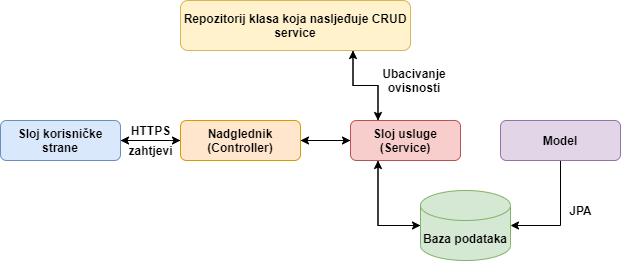
\includegraphics[scale=0.75]{slike/arhitektura.PNG} %veličina slike u odnosu na originalnu datoteku i pozicija slike
	\centering
	\caption{Spring Boot arhitektura}
	\label{fig:spring}
\end{figure}

Želimo li, radi lakšeg razumijevanja, našu arhitekturu usporediti sa stilom MVC (Model-View-Controller), možemo uočiti da se neki slojevi djelomično poklapaju. Primjerice sloj modela kod MVC-a
odgovarao bi sloju domene kod Spring Boota, sloj nadglednika kod MVC-a sloju
nadglednika kod Spring Boota, a sloj pogleda bio bi sloj korisničke strane. 


\vspace{15pt}
Kao što je navedeno, sloj korisničke strane (frontend) je implementiran u Java Scriptu koristeći knjižnicu React. \textbf{React} je besplatna biblioteka otvorenog koda za programski jezik JavaScript koja omogucava razvoj korisničkih sučelja SPA (eng. single-page application). SPA aplikacija je
tip web-aplikacije koja u interakciji s korisnikom dinamički mijenja dijelove stranice, za razliku od tradicionalnih web-aplikacija koje učitavaju cijele nove stranice s poslužitelja. One se pokreću u browseru i ne zahtijevaju ponovno učitavanje nakon korištenja.
React omogućava sastavljanje korisničkog sučelja pomoću elemenata koji se nazivaju komponente. Njih je mogucće iznova koristiti u aplikaciji proizvoljno veliki broj puta. Taj pristup pokazao se lakši za održavanje, proširivanje i višestruko korištenje.

\newpage



	
		

		

				
		\section{Baza podataka}
			
			U sklopu svih zahtjeva vezanih uz razvoj aplikacije nalaze se različiti entiteti i opisi veza među njima. Nijedno se najčešće ne zadaje eksplicitno, već se od inženjera očekuje da ih prepozna, nekako zapiše i pravilno implementira u svoj sustav. Kako bi sve te entitete prikazali na jednom mjestu te kako bi mogli pohranjivati informacije o njima važno je razviti dobru bazu podataka. Baza podataka za koju smo se odlučili u ovome projektu je relacijska; njen glavni objekt je relacija. Jedna relacija predstavlja jedan entitet. Svaka relacija je prikazana u obliku tablice koja ima svoje ime i atribute koji ju opisuju. Tablice su međusobno povezane pri čemu treba pripaziti na vrste veza među njima.  
			Baza podataka se sastoji od 6 glavnih entiteta:
			
			\begin{itemize}
				\item Walker 
				\item Shelter
				\item Walk
				\item Reservation
				\item Dog
				\item Location 
			\end{itemize}
		
			Značenje entiteta i opisi veza među njima su dani ispod. 
			
			\vspace{15pt}
			
			\subsection{Opis tablica}
			
			\vspace{10pt}
			
			\subsubsection{Walker}
			
				Tablica Walker predstavlja registriranog šetača/građana. Nakon što se korisnik aplikacije registrirao u sustavu, ili prijavio ukoliko već ima korisnički račun, on postaje registrirani šetač. Svaki registrirani šetač ima atribute poput imena, prezimena, adrese e-pošte i podataka za prijavu (korisničko ime i lozinka). Taj šetač ima opciju rezervacije termina i psa za šetnju. Iz tog razloga je povezan jedino s entitetom Reservation čija će uloga biti objašnjena ispod. Svaki šetač ima statistiku i raspored svojih šetnji. Ta dva entiteta nisu prepoznata kao zasebne tablice već kao potencijalni upiti nad rezervacijama koje je taj šetač napravio u sustavu. Važan atribut svakog šetača je statVisibility koji označava hoće li se šetačeva statistika šetanja vidjeti na javno dostupnoj rang listi. Svaki šetač ima opciju postavljanja te statistike kao javne ili privatne ovisno o vlastitim preferencijama. 
				
				\filbreak
				
				\begin{longtabu} to \textwidth {|X[6, l]|X[6, l]|X[20, l]|}
					
					\hline \multicolumn{3}{|c|}{\textbf{WALKER}}	 \\[3pt] \hline
					\endfirsthead
					
					\hline \multicolumn{3}{|c|}{\textbf{WALKER}}	 \\[3pt] \hline
					\endhead
					
					
					\hline 
					\endlastfoot
					
					\cellcolor{LightGreen}walkerId & INT	&  	Jedinstveni identifikator šetača 	\\ \hline
					firstName	& VARCHAR &  Ime šetača 	\\ \hline 
					lastName	& VARCHAR &  Prezime šetača 	\\ \hline 
					password & VARCHAR &  Hash lozinka šetača za login u sustav \\ \hline 
					email & VARCHAR &  Adresa e-pošte šetača \\ \hline 
					username & VARCHAR	&  Korisničko ime šetača		\\ \hline 
					statsVisibility	& BOOLEAN &  (Ne)vidljivost šetačeve statistike šetnji javno 	\\ \hline 
						
				\end{longtabu}
			
			\vspace{15pt}
			
			
			\subsubsection{Reservation}
			
				Tablica Reservation predstavlja logičku poveznicu između tri entiteta. Naime, svaki pas kojeg je šetač odabrao za neki termin biva zapisan u zasebnu rezervaciju. Na taj način je omogućeno da se različiti psi nalaze u šetnji kod istog šetača. Svaka rezervacija sadržava 4 atributa, svoj identifikator koji nam u pogledu razumijevanja modela ne znači previše i ostala 3 koja zapravo definiraju jednu rezervaciju.  Ti atributi su: walkId, walkerId i dogId. Zapisi (n-torke) u tablici rezervacija nam daju jasne informacije o tome koji šetači su šetali koje pse i u kojim terminima. Na taj način smo kreirali tablicu iz koje pomoću jednostavnih upita možemo doći do statistika šetnji, kako za pse tako i za šetače.  
			
			
				\begin{longtabu} to \textwidth {|X[6, l]|X[6, l]|X[20, l]|}
		
					\hline \multicolumn{3}{|c|}{\textbf{RESERVATION}}	 \\[3pt] \hline
					\endhead
					
					\hline \multicolumn{3}{|c|}{\textbf{RESERVATION}}	 \\[3pt] \hline
					\endhead
					
					\hline 
					\endlastfoot
					
					\cellcolor{LightGreen}reservationId & INT	&  	Jedinstveni identifikator rezervacije	\\ \hline
					\cellcolor{LightBlue} walkerId	& INT &  Jedinstveni identifikator šetača 	\\ \hline 
					\cellcolor{LightBlue} walkId & INT &  Jedinstveni identifikator šetnje \\ \hline 
					\cellcolor{LightBlue} dogId &INT	&  	Jedinstveni identifikator psa	\\ \hline 
					
				\end{longtabu}
			\newpage
			
			\subsubsection{Walk}
		
				Tablica Walk predstavlja jedan ugovoreni termin šetnje. Budući da je preko entiteta Reservation povezana s psima i šetačima, ne možemo direktno u n-torkama ove tablice vidjeti koji pas je sudjelovao u kojoj šetnji niti dobiti informaciju tko ga je šetao. Ukoliko poznajemo identifikator šetnje i ne koristimo druge tablice možemo saznati dvije informacije, a to su: datum i vrijeme početka i trajanje same šetnje. Kako bi se nova n-torka unijela u ovu tablicu nužno je da šetač napravi rezervaciju čime se implicitno podrazumijeva da se njen termin i ugovoreno trajanje tu zapisuje. 
		
				\begin{longtabu} to \textwidth {|X[6, l]|X[6, l]|X[20, l]|}
				
					\hline \multicolumn{3}{|c|}{\textbf{WALK}}	 \\[3pt] \hline
					\endfirsthead
					
					\hline \multicolumn{3}{|c|}{\textbf{WALK}}	 \\[3pt] \hline
					\endhead
					
					\hline 
					\endlastfoot
					
					\cellcolor{LightGreen}	walkId & INT &  Jedinstveni identifikator šetnje \\ \hline 
					dateTime	&TIMESTAMP &  Datum i vrijeme početka šetnje 	\\ \hline 
					duration & INT &  Duljina šetnje u minutama \\ \hline 
		
				\end{longtabu}
			
			\vspace{5pt}
			
			\subsubsection{Dog}
			
			
				Tablica Dog predstavlja psa. Svaki pas ima udrugu kojoj pripada, s time da je jasno da više pasa može pripadati istoj udruzi. Osim oznake kojoj udruzi pas pripada, on ima atribute koji označavaju njegovu lokaciju, ime, sliku i kratak opis. Osim toga svaki pas ima naznačeno koji tip šetnje preferira (grupne ili individualne). Individualna šetnja pretpostavlja da će jedan registrirani šetač rezervirati samo jednog psa za neki termin te će time napraviti jednu rezervaciju. Grupna šetnja označava situaciju u kojoj šetač odabire više pasa za isti termin te time radi onoliko rezervacija koliko je pasa odabrao. 
	
				\begin{longtabu} to \textwidth {|X[6, l]|X[6, l]|X[20, l]|}
				
					\hline \multicolumn{3}{|c|}{\textbf{DOG}}	 \\[3pt] \hline
					\endfirsthead
					
					\hline \multicolumn{3}{|c|}{\textbf{DOG}}	 \\[3pt] \hline
					\endhead
					
					\hline 
					\endlastfoot
					
					\cellcolor{LightGreen}dogId & INT	&  	Jedinstveni identifikator psa	\\ \hline
					image	& VARCHAR &   URI slike psa	\\ \hline 
					description & VARCHAR &  Opis psa \\ \hline 
					typeOfWalk & VARCHAR	&  	Tip šetnje za koju je pas predodređen (skupna/individualna)	\\ \hline 
					name	& VARCHAR & Ime psa  	\\ \hline 
					\cellcolor{LightBlue} shelterId &  INT	&  	Jedinstveni identifikator udruge	\\ \hline 
					\cellcolor{LightBlue} locationId & INT	&  	Jedinstveni identifikator lokacije	\\ \hline 
					
				
				\end{longtabu}
			
			
			\subsubsection{Shelter}
			
				Tablica Shelter predstavlja udrugu koja se u kontekstu aplikacije smatra drugom vrstom prijavljenog korisnika (osim već spomenutog šetača). Udruga ima svoj profil koji prikazuje slike i kratke opise pasa koji joj pripadaju. Osim informacije s kojim psima udruga raspolaže ona ima i svoje ime, OIB, lokaciju na kojoj se nalazi i naravno podatke za prijavu (korisničko ime i lozinku). Udruga raspolaže statistikom o šetnjama svojih pasa koja se također prikazuje na njenom profilu. Do te statistike se također dolazi putem pregleda svih rezervacija na kojima su njeni psi sudjelovali.   


				\begin{longtabu} to \textwidth {|X[6, l]|X[6, l]|X[20, l]|}
				
					\hline \multicolumn{3}{|c|}{\textbf{SHELTER}}	 \\[3pt] \hline
					\endfirsthead
					
					\hline \multicolumn{3}{|c|}{\textbf{SHELTER}}	 \\[3pt] \hline
					\endhead
					
					\hline 
					\endlastfoot
					
					\cellcolor{LightGreen}	shelterId &  INT	&  	Jedinstveni identifikator udruge	\\ \hline 
					password & VARCHAR &  Hash lozinka šetača za login u sustav \\ \hline 
					name	& VARCHAR &  Ime udruge	\\ \hline 
					username & VARCHAR	&  Korisničko ime udruge	\\ \hline 
					OIB	& VARCHAR &  OIB udruge	\\ \hline 
					\cellcolor{LightBlue} locationId & INT	&  	Jedinstveni identifikator lokacije	\\ \hline 
				
				\end{longtabu}
			
			
			\subsubsection{Location}
			
				Tablica Location predstavlja geografsku lokaciju. Tu lokaciju mogu imati udruge i psi. Pretpostavili smo da se dvije udruge neće nalaziti na istoj lokaciji budući da ju definiraju grad i točna adresa. No, više pasa može živjeti na istoj lokaciji te time ograničenje između broja pasa i lokacije ne postoji. Informacije o lokaciji udruge se nalaze na profilu udruge, dok se lokacija nekog psa vidi u slučaju da ga neki šetač želi rezervirati.
			
				\begin{longtabu} to \textwidth {|X[6, l]|X[6, l]|X[20, l]|}
					
					\hline \multicolumn{3}{|c|}{\textbf{LOCATION}}	 \\[3pt] \hline
					\endfirsthead
					
					\hline \multicolumn{3}{|c|}{\textbf{LOCATION}}	 \\[3pt] \hline
					\endhead
					
					\hline 
					\endlastfoot
					
					\cellcolor{LightGreen}	locationId &  INT	&  	Jedinstveni identifikator lokacije	\\ \hline 
					city & VARCHAR &  Grad \\ \hline 
					adress	& VARCHAR &  Adresa\\ \hline 
					
				\end{longtabu}
			
			
			\subsection{Dijagram baze podataka}
				
				\vspace{15pt} 
				\begin{figure}[H]
					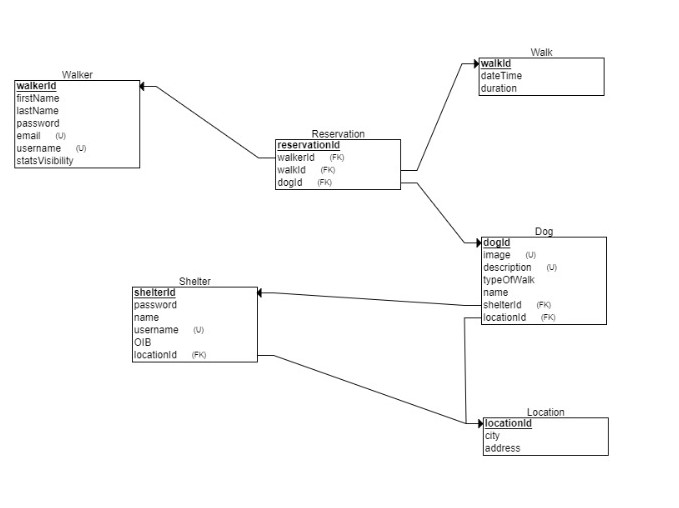
\includegraphics[scale=0.9]{dijagrami/relacijski.jpeg} %veličina slike u odnosu na originalnu datoteku i pozicija slike
					\centering
					\caption{Relacijski dijagram baze podataka}
					\label{fig:relacijski}
				\end{figure}
				\vspace{15pt}
			
			\eject
			
			
		\section{Dijagram razreda}
		
		\iffalse
			\textit{Potrebno je priložiti dijagram razreda s pripadajućim opisom. Zbog preglednosti je moguće dijagram razlomiti na više njih, ali moraju biti grupirani prema sličnim razinama apstrakcije i srodnim funkcionalnostima.}\\
			
			\textbf{\textit{dio 1. revizije}}\\
			
			\textit{Prilikom prve predaje projekta, potrebno je priložiti potpuno razrađen dijagram razreda vezan uz \textbf{generičku funkcionalnost} sustava. Ostale funkcionalnosti trebaju biti idejno razrađene u dijagramu sa sljedećim komponentama: nazivi razreda, nazivi metoda i vrste pristupa metodama (npr. javni, zaštićeni), nazivi atributa razreda, veze i odnosi između razreda.}\\
			
			\fi
			
			
			Na slikama su prikazani dijagrami razreda koji predstavljaju backend dio MVC arhitekture ostvarene korištenjem Java Spring Boota.
			
			\vspace{15pt} 
			\begin{figure}[H]
				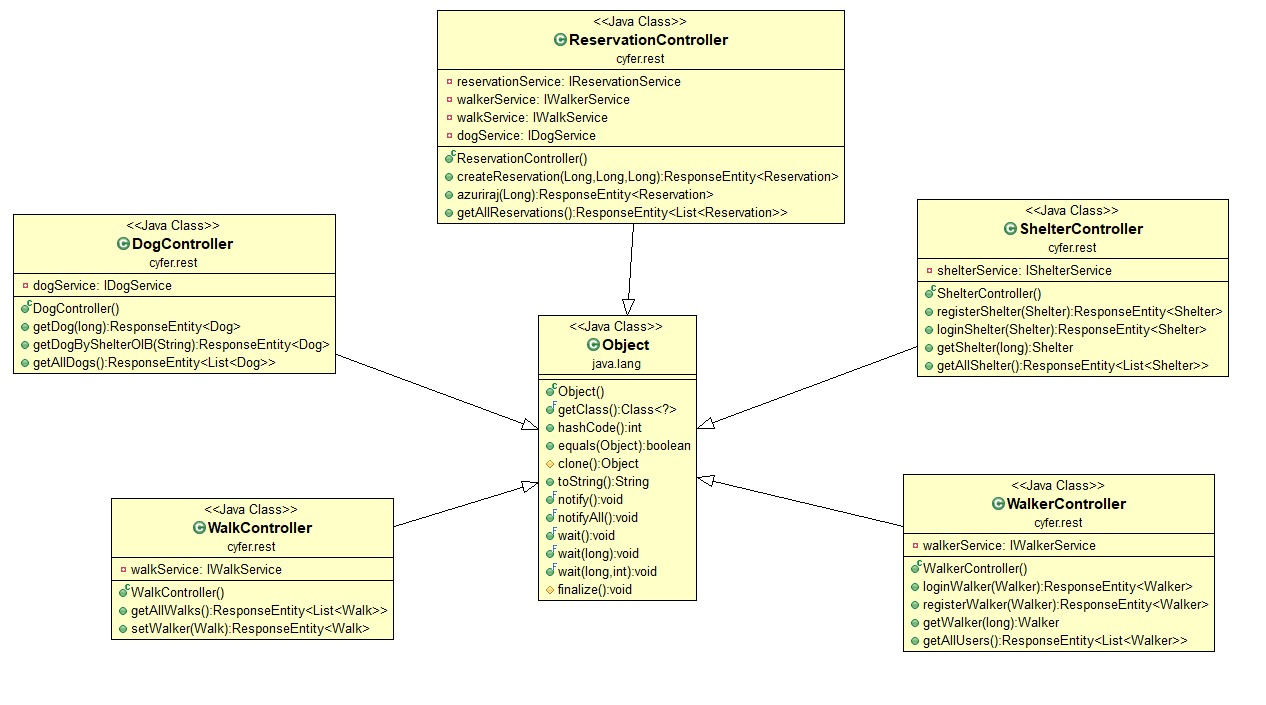
\includegraphics[scale=0.38]{dijagrami/controlleri.jpeg} %veličina slike u odnosu na originalnu datoteku i pozicija slike
				\centering
				\caption{Razredi controlleri}
				\label{fig:controlleri}
			\end{figure}
			
			
			Razredi prikazani na slici ~\ref{fig:controlleri} predstavljaju MVC Kontrolere čije metode mapiraju određene zahtjeve putem URI-a, te vraćaju JSON datoteke koje se potom obrađuju na određeni način. Također šalju i HTML statusni kod.
			Kontroleri su implementirani za pet klasa tipa Model: Dog, Walk, Shelter, Walker i Reservation. Svaki razred ima konstruktor i metode koje mapiraju određene zahtjeve zadanim HTTP zahtjevom.
			
				\vspace{15pt} 
			\begin{figure}[H]
				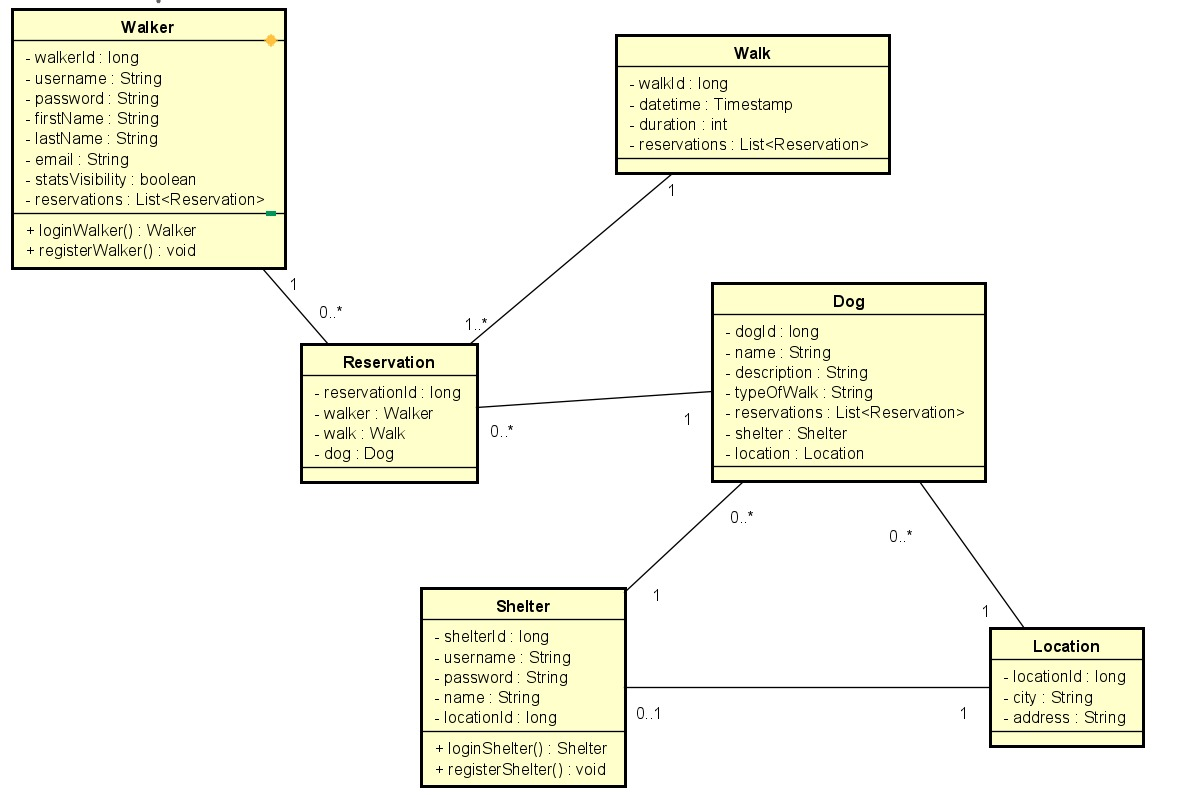
\includegraphics[scale=0.4]{dijagrami/modeli.jpeg} %veličina slike u odnosu na originalnu datoteku i pozicija slike
				\centering
				\caption{Razredi modeli}
				\label{fig:modeli}
			\end{figure}
			
			
		Razredi prikazani na slici ~\ref{fig:modeli} predstavljaju MVC Modele koji odgovaraju entitetima u bazi podataka. Svaki razred sadrži svoj konstruktor, privatne članske varijable koje su mu svojstvene i koje odgovaraju atributima u bazi, kao i sve gettere i settere.
		Razred Dog predstavlja psa koji je pridruženoj određenoj udruzi (Shelter) i dostupan je za šetnje. Razred Walker predstavlja registriranog korisnika (šetača) koji može odabrati psa/pse za šetnju. Razred Shelter predstavlja registriranu udrugu koja ima svoj profil i pse dostupne za šetnju. Razred Walk predstavlja šetnju koja se dogodila s jednim šetačom i jednim ili više pasa. Razred Location predstavlja lokaciju (grad i adresa) na kojoj može biti smješten pas ili udruga. Kardinalnosti veza među razredima su prikazane na dijagramu.
			
			
			\iffalse
			\textbf{\textit{dio 2. revizije}}\\			
			
			\textit{Prilikom druge predaje projekta dijagram razreda i opisi moraju odgovarati stvarnom stanju implementacije}
			
			\fi
			
			\eject
		
		\section{Dijagram stanja}
			
			
			\textbf{\textit{dio 2. revizije}}\\
			
			\textit{Potrebno je priložiti dijagram stanja i opisati ga. Dovoljan je jedan dijagram stanja koji prikazuje \textbf{značajan dio funkcionalnosti} sustava. Na primjer, stanja korisničkog sučelja i tijek korištenja neke ključne funkcionalnosti jesu značajan dio sustava, a registracija i prijava nisu. }
			
			
			\eject 
		
		\section{Dijagram aktivnosti}
			 \textit
			Korisnik upisuje podatke za prijavu. Poslužitelj dohvaća podatke o registriranim korisnicima iz baze podataka te provjerava postoji li korisnik u bazi. Ako ne postoji, vraća poruku o neuspješnoj prijavi. Ako postoji, preusmjerava korisnika na stranicu za registrirane korisnike. Korisnik s te stranice odabire stranicu profila. Poslužitelj dohvaća podatke o korisniku iz baze te ih prikazuje. Korisnik odabire opciju pregleda kalendara sa šetnjama. Poslužitelj iz baze dohvaća podatke o rezerviranim šetnjama korisnika i prikazuje kalendar sa svim rezerviranim šetnjama.
			\newpage
			\begin{figure}[H]
				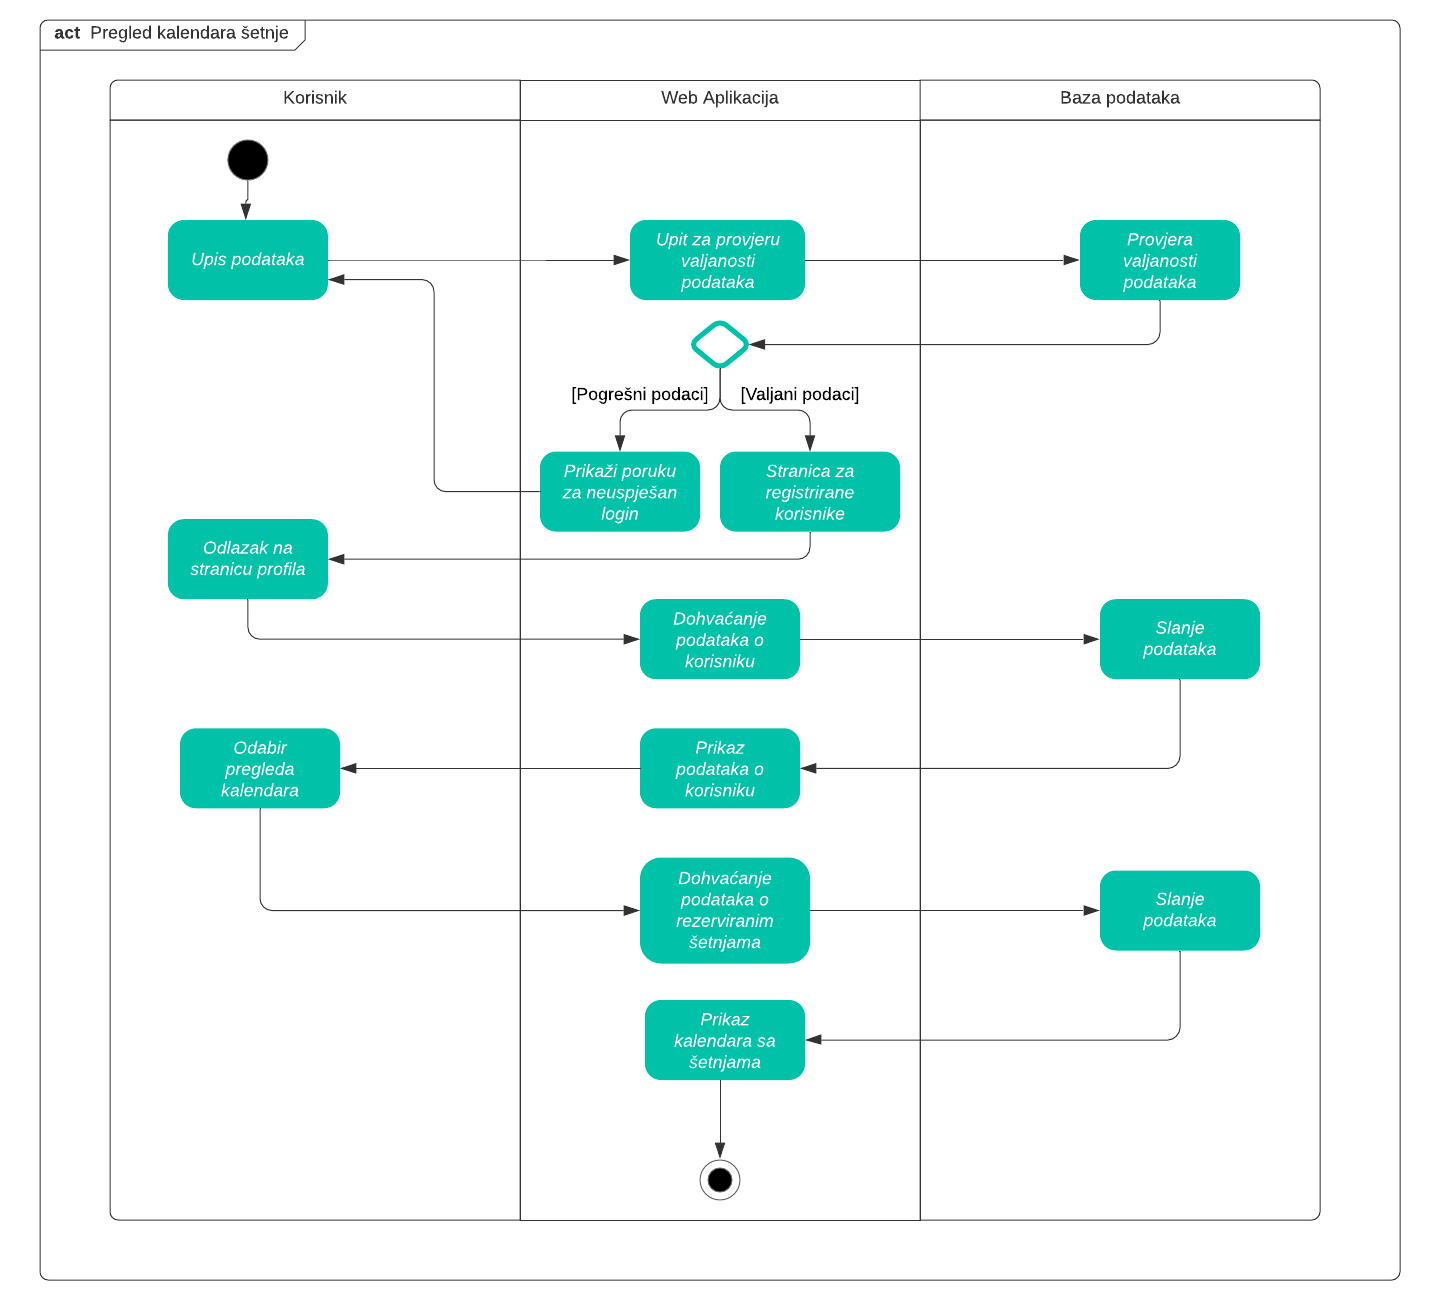
\includegraphics[width=1\textwidth]{dijagrami/act.png} %veličina u odnosu na širinu linije
				\caption{Dijagram aktivnosti: Pregled kalendara šetnje}
				\label{fig:Act1} %label mora biti drugaciji za svaku sliku
			\end{figure}
		
			\newpage
			\eject
		\section{Dijagram komponenti}
		
			\textbf{\textit{dio 2. revizije}}\\
		
			 \textit{Potrebno je priložiti dijagram komponenti s pripadajućim opisom. Dijagram komponenti treba prikazivati strukturu cijele aplikacije.}
	\chapter{Implementacija i korisničko sučelje}
		
		
		\section{Korištene tehnologije i alati}
		
			\textbf{\textit{dio 2. revizije}}
			
			 \textit{Detaljno navesti sve tehnologije i alate koji su primijenjeni pri izradi dokumentacije i aplikacije. Ukratko ih opisati, te navesti njihovo značenje i mjesto primjene. Za svaki navedeni alat i tehnologiju je potrebno \textbf{navesti internet poveznicu} gdje se mogu preuzeti ili više saznati o njima}.
			
			
			\eject 
		
	
		\section{Ispitivanje programskog rješenja}
			
			
			\subsection{Ispitivanje komponenti}
			Testirali smo 8 ispitnih slučajeva unoseći ispravne i neispravne podatke te provjeravajući vraća li sustav odgovore kakve očekujemo. Od osam ispitnih primjera, četiri se odnose na šetače te četiri na udruge. Rezultati i opisi pojedinih testova su priloženi ispod. Kao što ćemo vidjeti u rezultatima, svi su ispiti prolazni jer smo pri upisu neispravnih podataka i očekivali odgovore različite od 200 OK.
			
			\subsubsection{1. ispitni primjer - registracija udruge sa zauzetim OIB-om}
			
			U ispitnom primjeru prvo smo stvorili i registrirali prvu udrugu sa zadanim OIB-om 22000000000. Dobili smo očekivani odgovor sa statusom 200 OK. Zatim smo pokušali registrirati drugu udrugu sa istim tim OIB-om (ali drugačijim korisničkim imenom, koji također mora biti jedinstven). Dobili smo očekivani odgovor sa statusom 406 NOT ACCEPTABLE. Nakon toga smo promijenili OIB u 22000000001 te ponovno poslali zahtjev za registracijom. Dobili smo očekivani odgovor 200 OK.
			\begin{figure}[H]
				\centerline{
					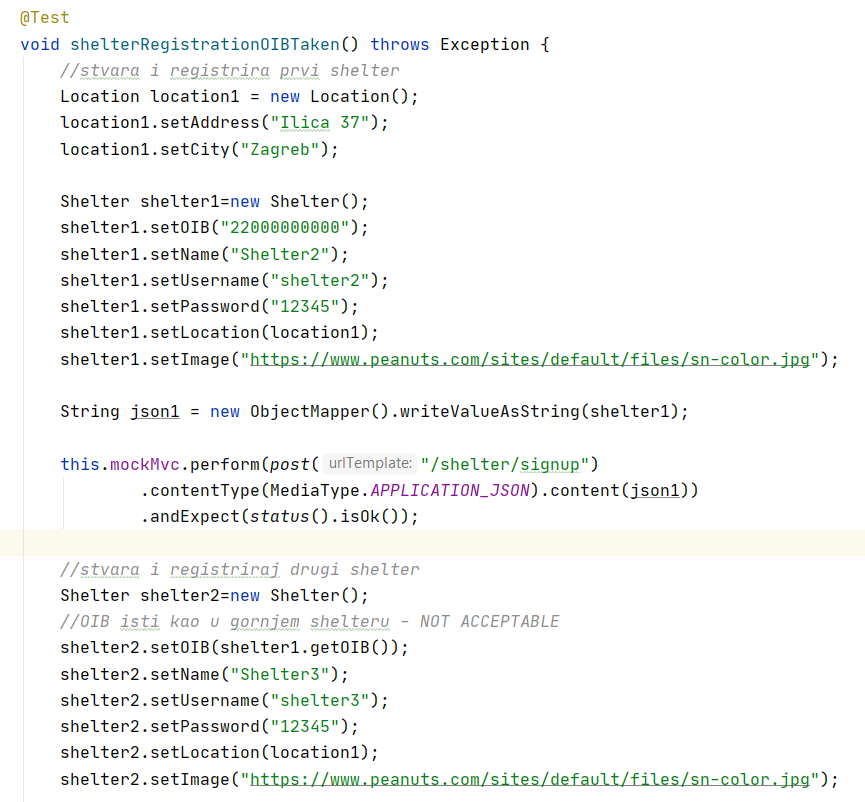
\includegraphics[scale=0.73]{slike/shelter1.1.PNG}}
				\hspace*{-0.21in}
				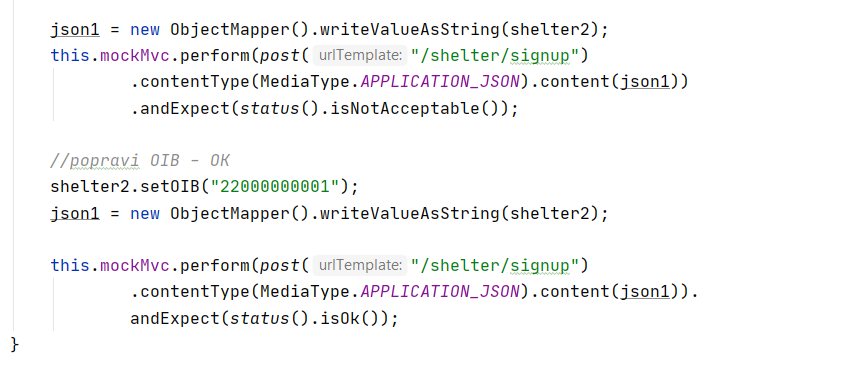
\includegraphics[scale=0.73]{slike/shelter1.2.PNG}
				%veličina slike u odnosu na originalnu datoteku i pozicija slike
				\centering
			\end{figure}
			
			
			
			\subsubsection{2. ispitni primjer - registracija udruge sa zauzetim korisničkim imenom}
			
			U ispitnom primjeru prvo smo stvorili i registrirali prvu udrugu sa zadanim korisničkim imenom "ella". Dobili smo očekivani odgovor sa statusom 200 OK. Zatim smo pokušali registrirati drugu udrugu sa istim tim korisničkim imenom (ali drugačijim OIB-om, koji također mora biti jedinstven). Dobili smo očekivani odgovor sa statusom 409 CONFLICT. Možemo primjetiti da je to drugačiji odgovor od onog u gornjem testu kada šaljemo OIB koji nije jedinstven (409 NOT ACCEPTED). To je zato što smo pomoću tih odgovora razlikovali kakav odgovor tj. feedback treba dati korisniku pri registraciji. Nakon toga smo promijenili korisničko ime u "lily" te ponovno poslali zahtjev za registracijom. Dobili smo očekivani odgovor 200 OK.
			
			\begin{figure}[H]
				\centerline{
					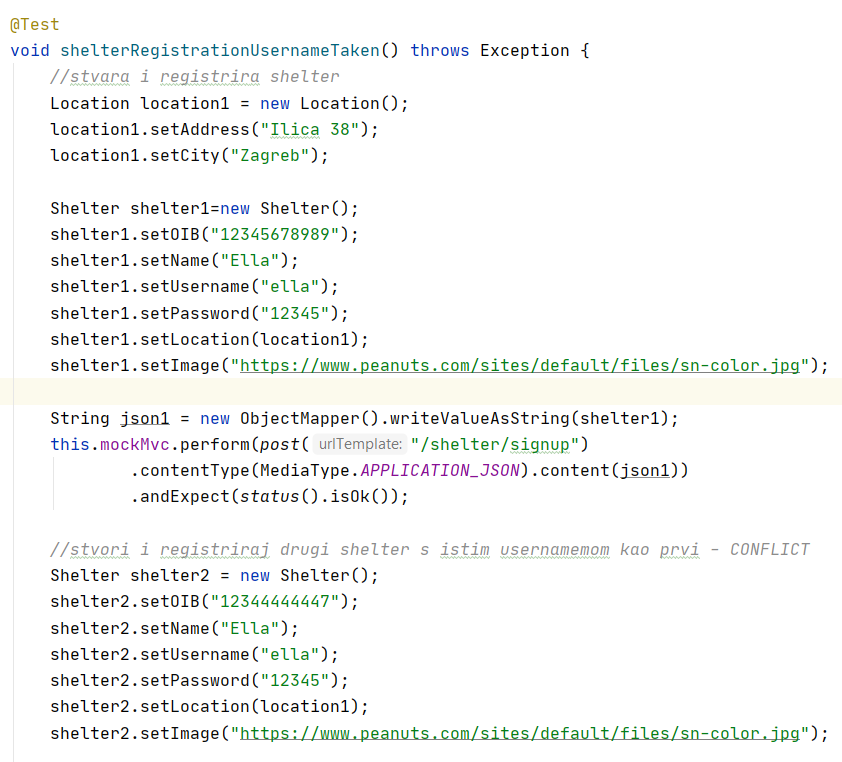
\includegraphics[scale=0.75]{slike/shelter2.1.PNG}}
				\hspace*{-0.22in}
				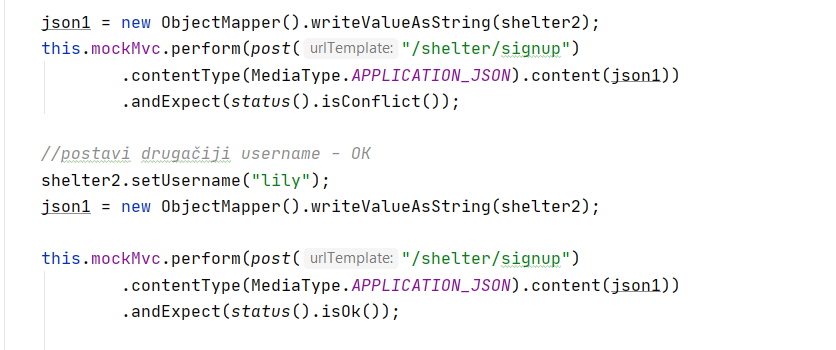
\includegraphics[scale=0.75]{slike/shelter2.2.PNG} %veličina slike u odnosu na originalnu datoteku i pozicija slike
				\centering
			\end{figure}
			
			
			
			\subsubsection{3. ispitni primjer - mijenjanje podataka udruge sa i bez autorizacije }
			
			U ispitnom primjeru prvo smo stvorili i registrirali  udrugu. Dobili smo očekivani odgovor sa statusom 200 OK. Također, u tijelu odgovora nam je vraćena ta udruga koju smo upravo registrirali uz dodatak ID-a udruge koji je stvoren na backendu. Taj vraćeni objekt smo spremili u našu varijablu udruge jer ćemo koristiti vraćeni ID u putanji za mijenjanje podataka. Zatim smo promijenili ime udruge u "NovoIme" te poslali zahtjev za promjenom. Dobili smo očekivani odgovor sa statusom 401 UNAUTHORIZED jer nismo dodali autorizaciju na zahtjev. Nakon toga smo pokušali ponovno sa dodanom autorizacijom te dobili očekivani odgovor 200 OK te udrugu sa promijenjenim imenom u tijelu odgovora. Na kraju smo provjerili da je u vraćenoj udruzi stvarno promijenjeno ime.
			
			\begin{figure}[H]
				\hspace*{-0.5in}
				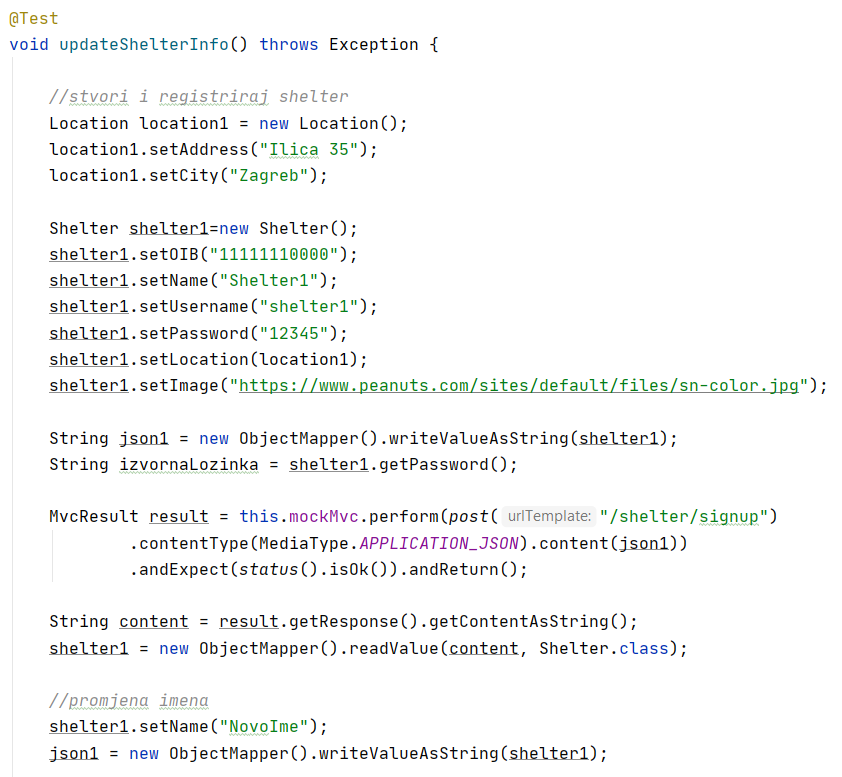
\includegraphics[scale=0.73]{slike/shelter3.1.PNG}
				\hspace*{-0.45in}	
				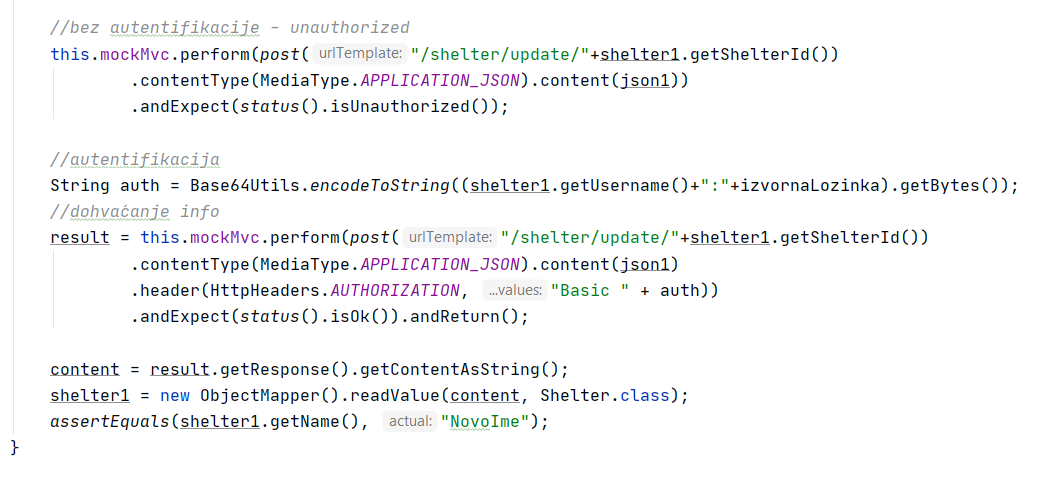
\includegraphics[scale=0.73]{slike/shelter3.2.PNG} %veličina slike u odnosu na originalnu datoteku i pozicija slike
				\centering
			\end{figure}
			
			
			\subsubsection{4. ispitni primjer - brisanje udruge sa i bez autorizacije }
			
			U ispitnom primjeru prvo smo stvorili i registrirali  udrugu. Dobili smo očekivani odgovor sa statusom 200 OK. Također, u tijelu odgovora nam je vraćena ta udruga koju smo upravo registrirali uz dodatak ID-a udruge koji je stvoren na backendu. Taj vraćeni objekt smo spremili u našu varijablu udruge jer ćemo koristiti vraćeni ID u putanji za brisanje udruge. Zatim smo poslali zahtjev za brisanjem bez autorizacije. Dobili smo očekivani odgovor sa statusom 401 UNAUTHORIZED jer nismo dodali autorizaciju na zahtjev. Nakon toga smo pokušali ponovno sa dodanom autorizacijom te dobili očekivani odgovor 200 OK.
			
			\begin{figure}[H]
				\hspace*{-0.93in}
				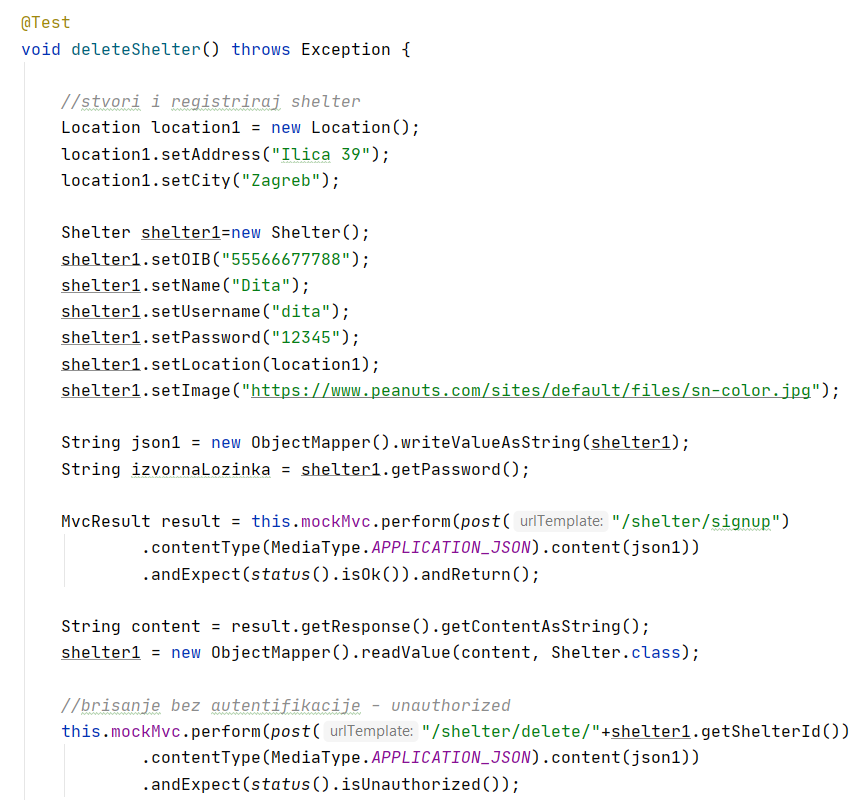
\includegraphics[scale=0.71]{slike/shelter4.1.PNG}
				\hspace*{-0.6in}
				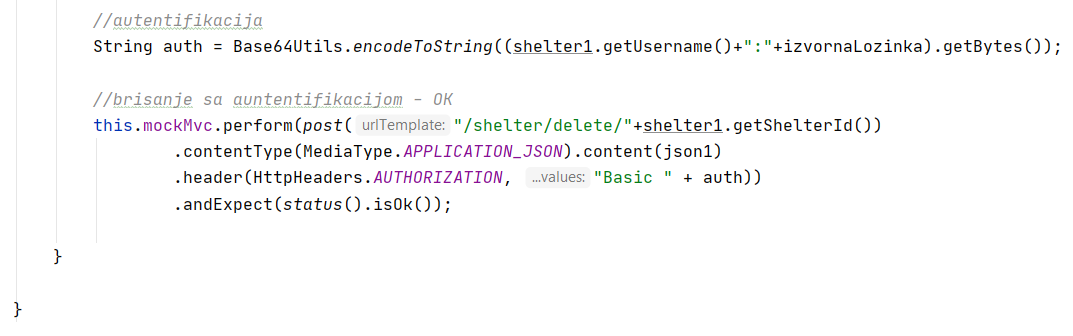
\includegraphics[scale=0.71]{slike/shelter4.2.PNG} %veličina slike u odnosu na originalnu datoteku i pozicija slike
				\centering
			\end{figure}
			
			
			
			\subsubsection{5. ispitni primjer - registracija šetača sa zauzetom email adresom}
			
			U ispitnom primjeru prvo smo stvorili dva šetača sa jednakim email adresama (ali različitim korisničkim imenima, koja također moraju biti jedinstvena). Registrirali smo prvog i dobili očekivani odgovor sa statusom 200 OK. Zatim smo pokušali registrirati drugog šetača te smo dobili  očekivani odgovor sa statusom 406 NOT ACCEPTABLE jer email adresa šetača mora biti jedinstvena.
			
			
			\begin{figure}[H]
				\centerline{
					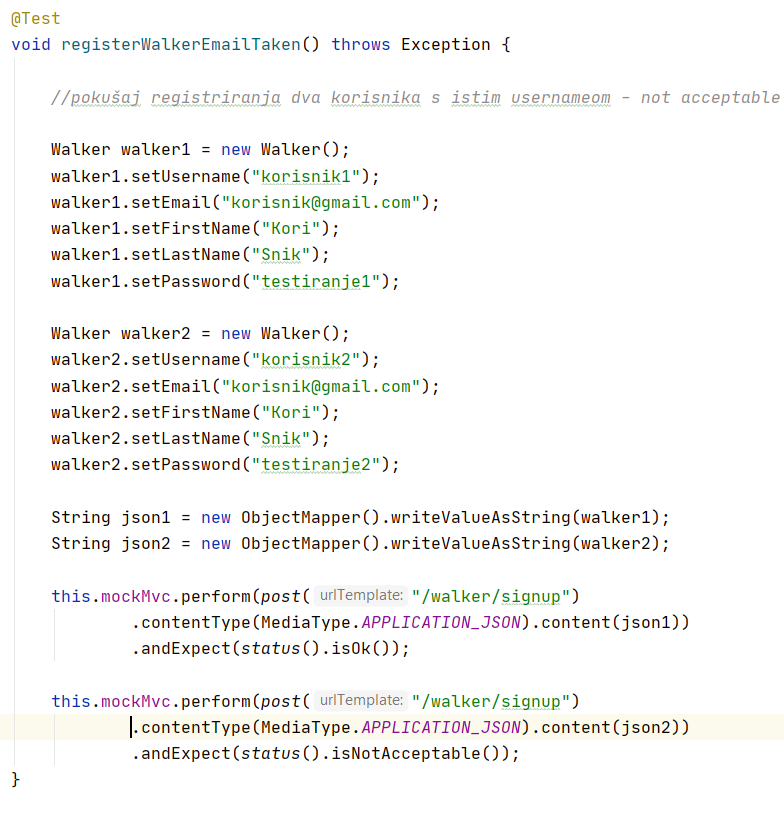
\includegraphics[scale=0.75]{slike/walker1.PNG}}
				%veličina slike u odnosu na originalnu datoteku i pozicija slike
				\centering
			\end{figure}
			
			\newpage
				
			\subsubsection{6. ispitni primjer - registracija šetača sa zauzetim korisničkim imenom}
			
			U ispitnom primjeru prvo smo stvorili dva šetača sa jednakim korisničkim imenom (ali različitim email adresama, koje također moraju biti jedinstvene). Registrirali smo prvog i dobili očekivani odgovor sa statusom 200 OK. Zatim smo pokušali registrirati drugog šetača te smo dobili  očekivani odgovor sa statusom 409 CONFLICT jer e korisničko ime šetača mora biti jedinstveno. Kao i u primjeru s udrugama, šaljemo različite statuse ovisno je li došlo do pogreške zbog korisničkog imena ili lozinke jer tako znamo kakvu poruku poslati korisniku.
			
			
			\begin{figure}[H]
				\centerline{
					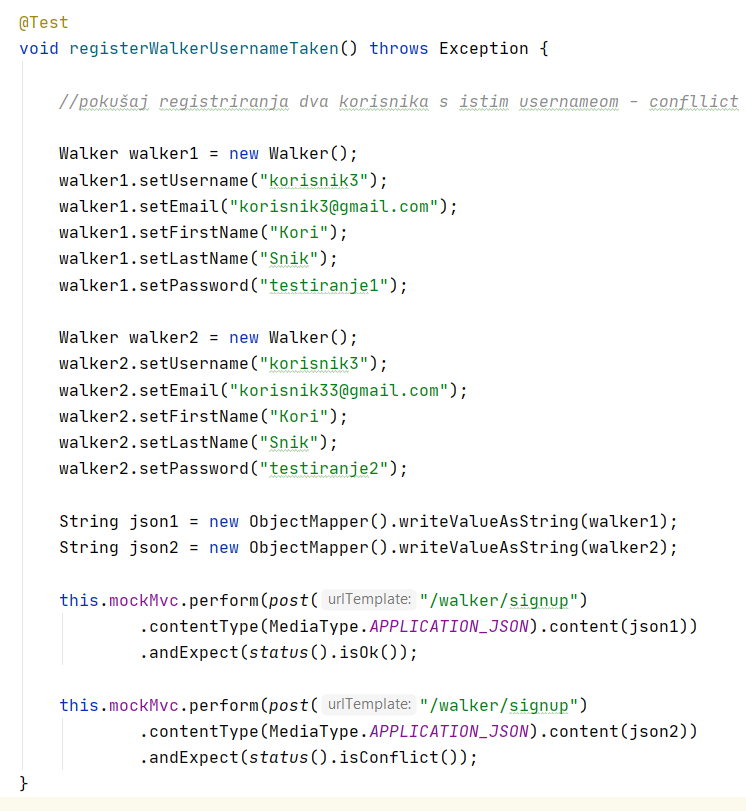
\includegraphics[scale=0.75]{slike/walker2.PNG}} %veličina slike u odnosu na originalnu datoteku i pozicija slike
				\centering
			\end{figure}
			
			
			\subsubsection{7. ispitni primjer - mijenjanje podataka šetača sa i bez autorizacije }
			
			U ispitnom primjeru prvo smo stvorili i registrirali  šetača. Dobili smo očekivani odgovor sa statusom 200 OK. Također, u tijelu odgovora nam je vraćen taj šetač kojeg smo upravo registrirali uz dodatak ID-a šetača koji je stvoren na backendu. Taj vraćeni objekt smo spremili u našu varijablu šetača jer ćemo koristiti vraćeni ID u putanji za mijenjanje podataka. Zatim smo promijenili korisničko ime šetača u "noviKorisnik" te poslali zahtjev za promjenom. Dobili smo očekivani odgovor sa statusom 401 UNAUTHORIZED jer nismo dodali autorizaciju na zahtjev. Nakon toga smo pokušali ponovno sa dodanom autorizacijom te dobili očekivani odgovor 200 OK te šetača sa promijenjenim korisničkim imenom u tijelu odgovora. Na kraju smo provjerili da je vraćenom šetaču stvarno promijenjeno ime.
			
			
			
			\begin{figure}[H]
				\hspace*{-0.58in}
				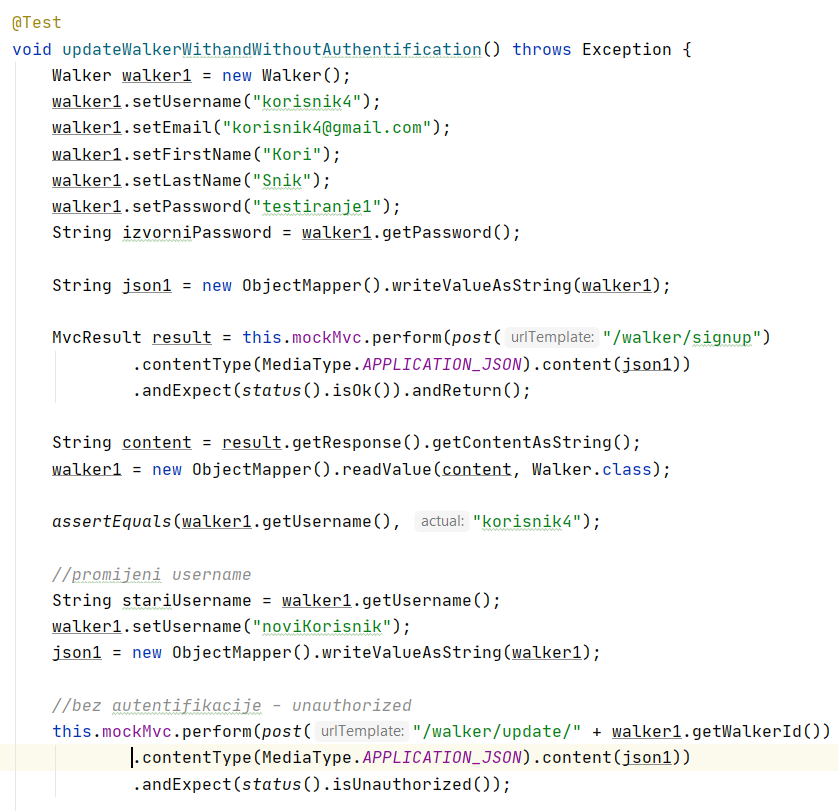
\includegraphics[scale=0.73]{slike/walker3.1.PNG}
				\hspace*{-0.41in}
				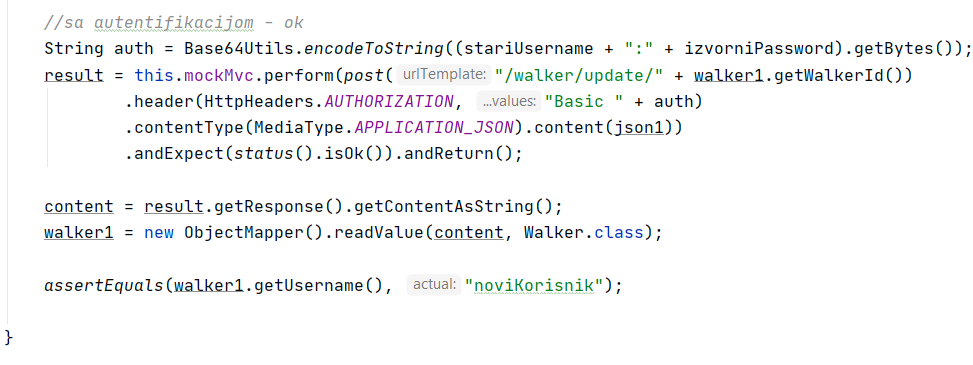
\includegraphics[scale=0.73]{slike/walker3.2.PNG} %veličina slike u odnosu na originalnu datoteku i pozicija slike
				\centering
			\end{figure}
			
			
			\subsubsection{8. ispitni primjer - mijenjanje podataka šetača sa i bez autorizacije }
			
			U ispitnom primjeru prvo smo stvorili i registrirali  šetača. Dobili smo očekivani odgovor sa statusom 200 OK.  Zatim smo stvorili novu šetnju te poslali zahtjev za rezervacijom šetnje (odabrali smo psa sa ID-jem 13 i stavili 13 u stazu "/reserve/13"). Dobili smo očekivani odgovor sa statusom 401 UNAUTHORIZED jer nismo dodali autorizaciju na zahtjev. Nakon toga smo pokušali ponovno sa dodanom autorizacijom te dobili očekivani odgovor 200 OK. 
			
			
			\begin{figure}[H]
				\hspace*{-0.18in}
				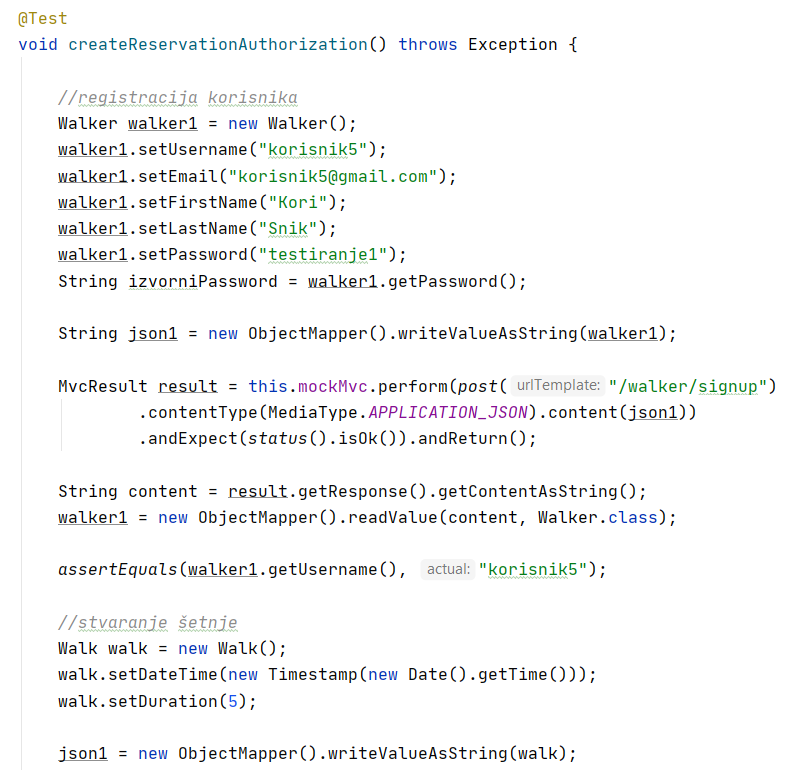
\includegraphics[scale=0.75]{slike/walker4.1.PNG}
				\hspace*{-0.4in}
				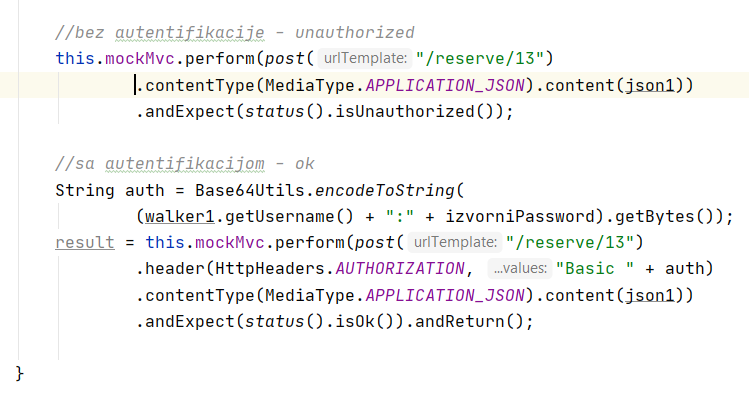
\includegraphics[scale=0.75]{slike/walker4.2.PNG} %veličina slike u odnosu na originalnu datoteku i pozicija slike
				\centering
			\end{figure}
		
		
			\subsubsection{Rezultati ispitnih primjera }
			
			\begin{figure}[H]
				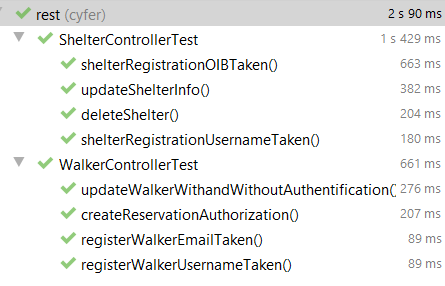
\includegraphics[scale=0.75]{slike/UnitRezultati.PNG}
				\centering
			\end{figure}
			
			
			
			
			\subsection{Ispitivanje sustava}
			
				Za ispitivanje sustava koristili smo radni okvir Selenium. Uz podršku Selenium WebDrivera, napisali smo četiri ispita u programskom jeziku Java. Kao i u gornjim primjerima, svi ispiti su uspješno prošli jer smo pri slanju krivih podataka očekivali da su korisniku prikazane informacije o tome što je krivo. Svi ispiti su vezani uz varijacije registracija šetača i udruge. Očekivali smo da sustav zna reći koji podaci su neispravni kako bi ih mogao ispraviti.
			
			\subsubsection{1. ispitni primjer - registracija šetača sa ispravnim podatcima}
			
				U ovom primjeru smo demonstrirali uspješnu registraciju šetača. Od sustava smo očekivali da nas onda preusmjeri na početnu stranicu, što je ispunjeno.
				
			 	\begin{figure}[H]
			 	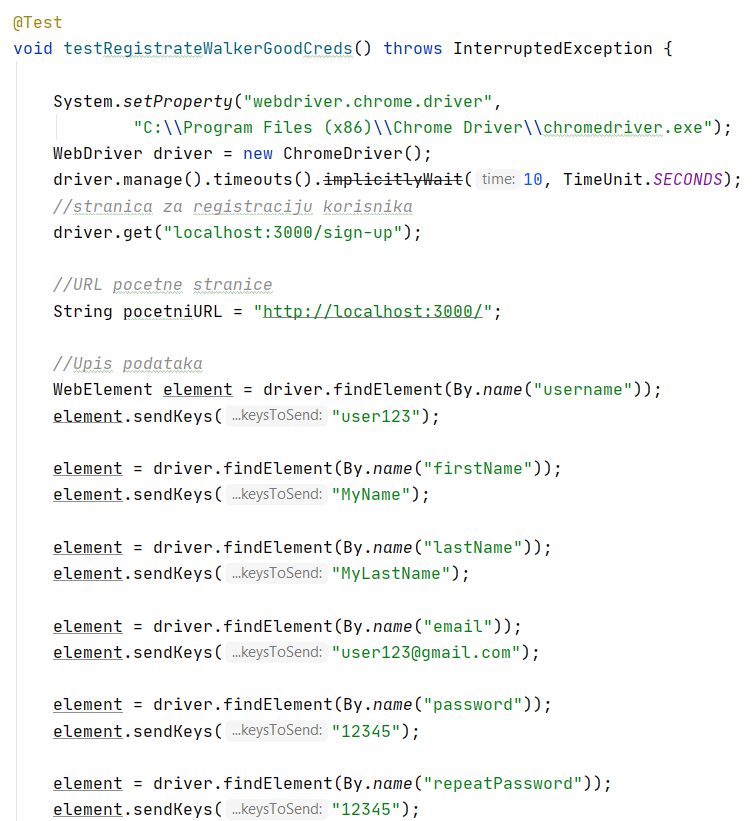
\includegraphics[scale=0.75]{slike/Selenium1.1.PNG}
			 	\hspace*{-0.85in}
			 	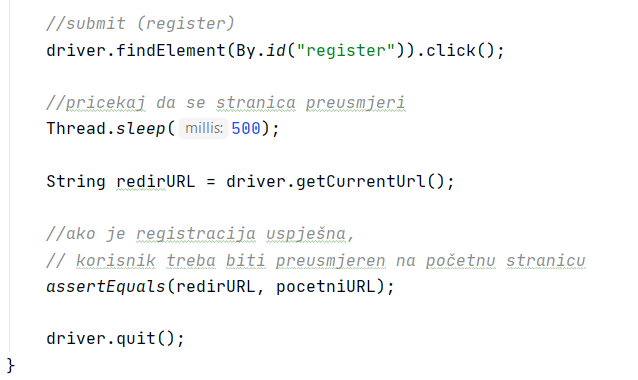
\includegraphics[scale=0.75]{slike/Selenium1.2.PNG} %veličina slike u odnosu na originalnu datoteku i pozicija slike
			 	\centering
			 \end{figure}
		 
		 
		 
		 \subsubsection{2. ispitni primjer - registracija šetača s neispravnim podatcima}
		 
		 U ovom primjeru smo demonstrirali neuspješnu registraciju šetača. Upisali smo isto korisničko ime kao i u gornjem primjeru - "user123", a kako smo ispite pokretali slijedno, takav korisnik je već bio u bazi. Od sustava smo očekivali da nam javi kakva je pogreška u pitanju. Sustav je ostao na istoj stranici (nije se dogodilo preusmjeravanje kao pri uspješnoj registraciji) te nam je ispisao poruku "Neuspješna registracija - korisničko ime je zauzeto." U ispitnom primjeru smo provjerili je li doista ispisana ta poruka. Ispod je priložena slika izvođenja u browseru te kod ispitnog primjera. 
		 
		 	\begin{figure}[H]
		 		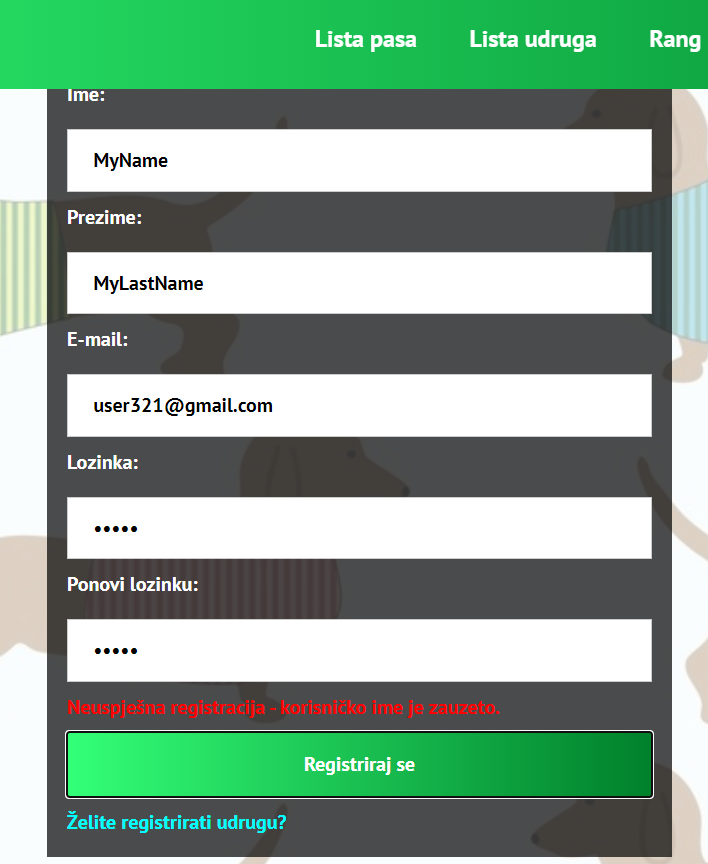
\includegraphics[scale=0.70]{slike/UsernameError.PNG}
		 		 %veličina slike u odnosu na originalnu datoteku i pozicija slike
		 		\centering
		 	\end{figure}
			 
			 \begin{figure}[H]
			 	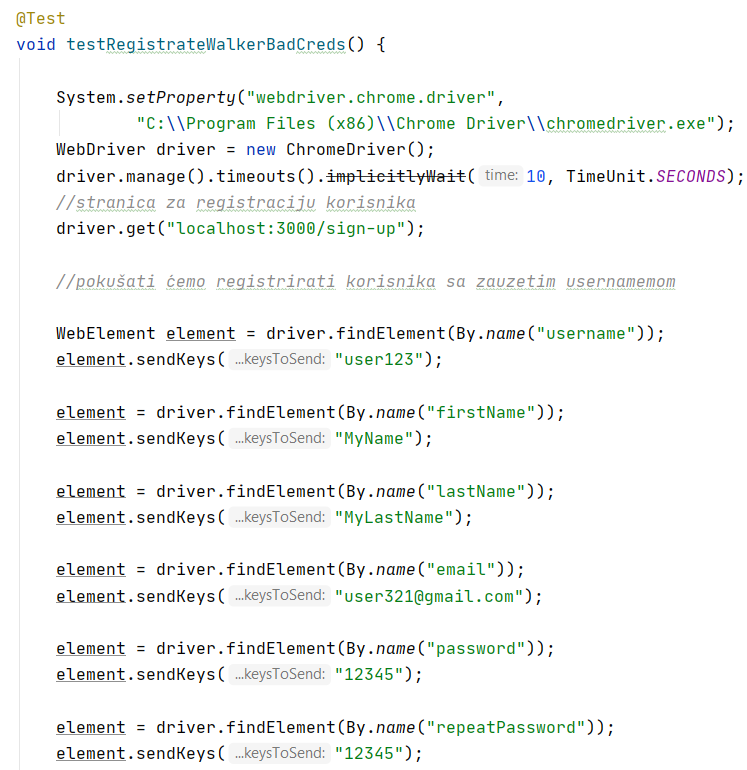
\includegraphics[scale=0.75]{slike/Selenium2.1.PNG}
			 	\hspace*{0.15in}
			 	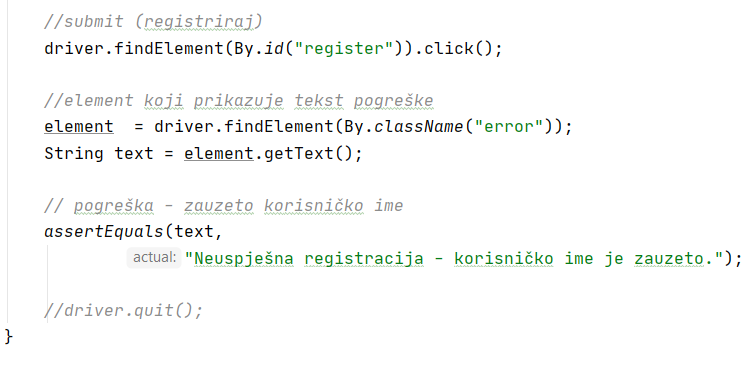
\includegraphics[scale=0.75]{slike/Selenium2.2.PNG} %veličina slike u odnosu na originalnu datoteku i pozicija slike
			 	\centering
			 \end{figure}
		 
		 
		   \subsubsection{3. ispitni primjer - registracija udruge sa ispravnim podatcima}
		 
		 U ovom primjeru smo demonstrirali uspješnu registraciju udruge uz ispravak lozinke. Upisali smo sve ispravne podatke osim lozinke i ponovljene lozinke, koje su bile različite. Od sustava smo očekivali da nam javi kakva je pogreška u pitanju. Sustav je ostao na istoj stranici (nije se dogodilo preusmjeravanje kao pri uspješnoj registraciji) te nam je ispisao poruku "Lozinke se ne poklapaju." Zatim smo ispravili ponovljenu lozinku i ponovno poslali zahtjev za registracijom. Sustav nas je očekivano preusmjerio na početnu stranicu. Ispod je priložena slika izvođenja u browseru (neispravne lozinke) te kod ispitnog primjera. 
			 
			  \begin{figure}[H]
			 	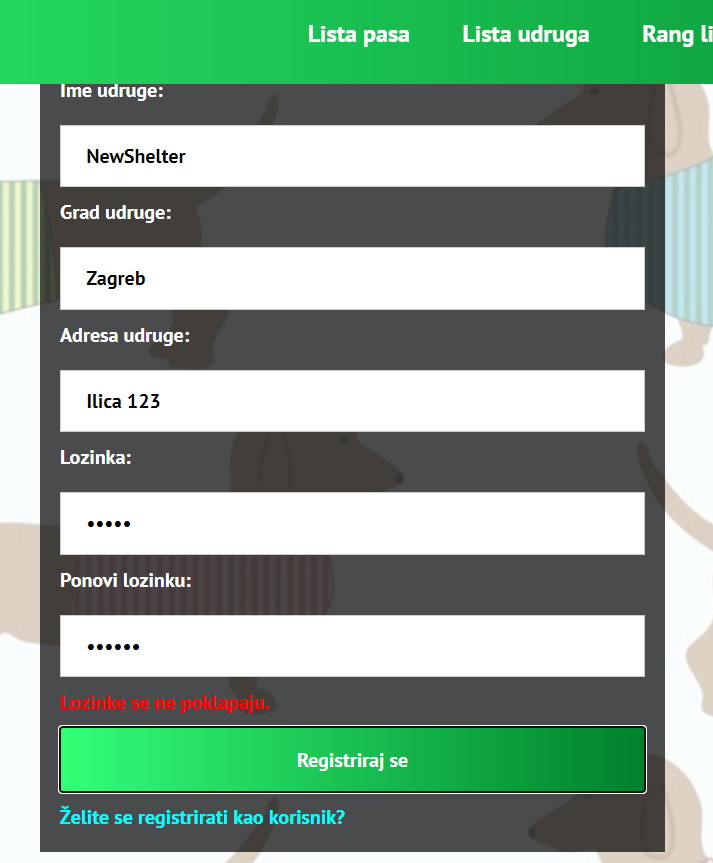
\includegraphics[scale=0.75]{slike/PasswordError.PNG}
			 	%veličina slike u odnosu na originalnu datoteku i pozicija slike
			 	\centering
			 \end{figure}
			 \begin{figure}[H]
			 	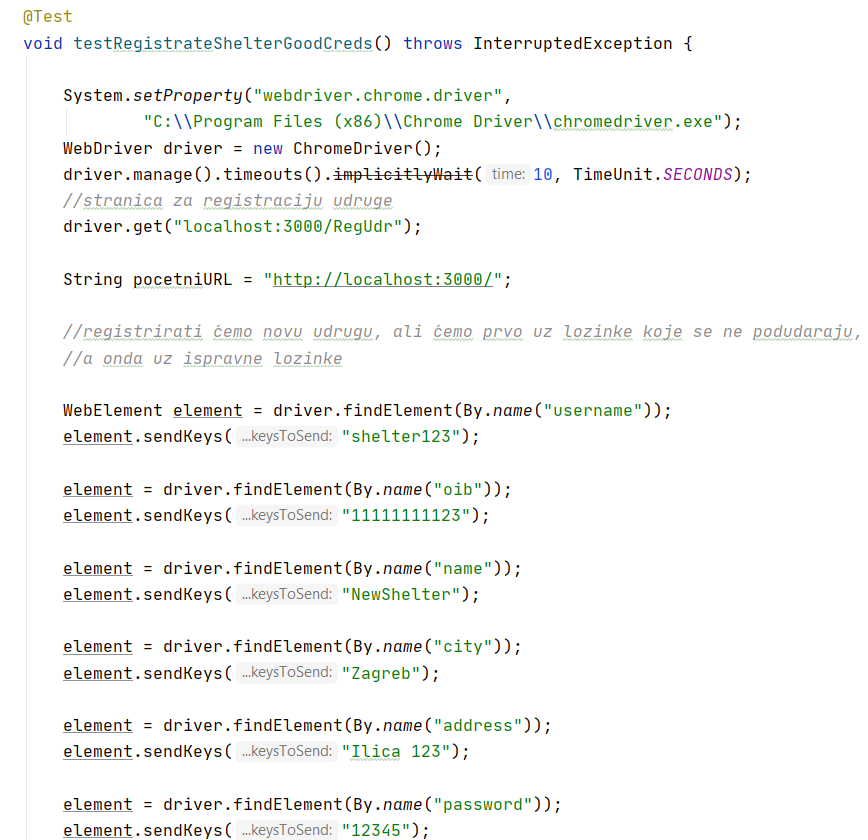
\includegraphics[scale=0.75]{slike/Selenium3.1.PNG}
			 	%veličina slike u odnosu na originalnu datoteku i pozicija slike
			 	\centering
			 \end{figure}
			 \begin{figure}[H]
			 	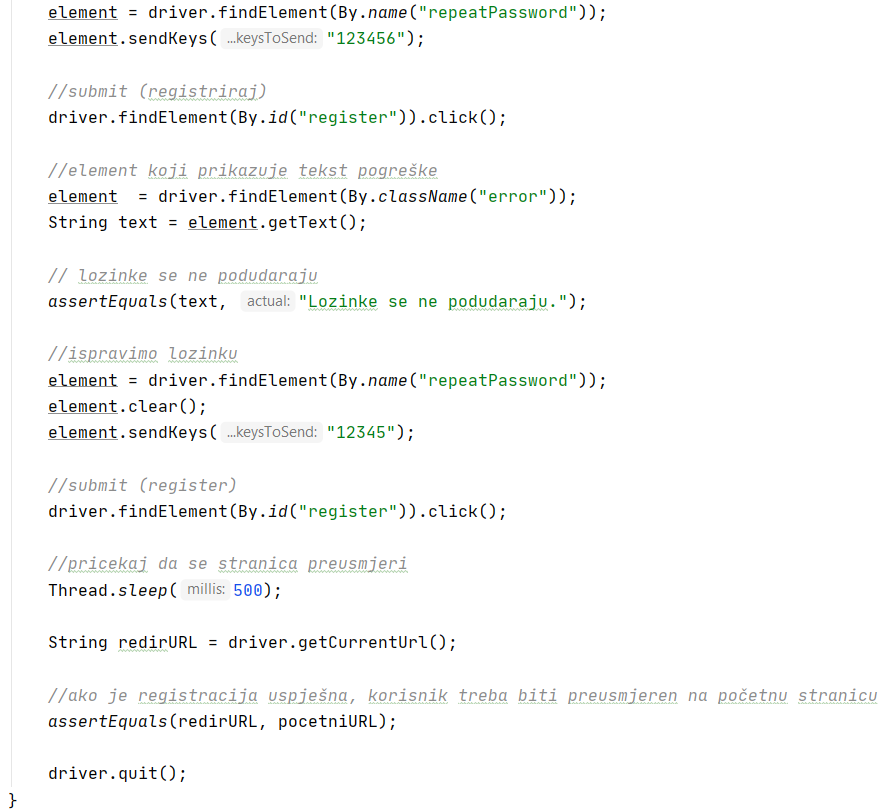
\includegraphics[scale=0.75]{slike/Selenium3.2.PNG} %veličina slike u odnosu na originalnu datoteku i pozicija slike
			 	\centering
			 \end{figure}
			 
			 
			 
			  \subsubsection{4. ispitni primjer - registracija udruge s neispravnim podatcima}
			 
			 U ovom primjeru smo demonstrirali neuspješnu registraciju udruge. Upisali smo isti OIB kao i u gornjem (trećem) primjeru - "11111111123", a kako smo ispite pokretali slijedno, takva udruga je već bila u bazi. Od sustava smo očekivali da nam javi kakva je pogreška u pitanju. Sustav je ostao na istoj stranici (nije se dogodilo preusmjeravanje kao pri uspješnoj registraciji) te nam je ispisao poruku "Neuspješna registracija - postoji već udruga sa danim OIB-om." U ispitnom primjeru smo provjerili je li doista ispisana ta poruka. Ispod je priložena slika izvođenja u browseru te kod ispitnog primjera. 
			 
			 \begin{figure}[H]
			 	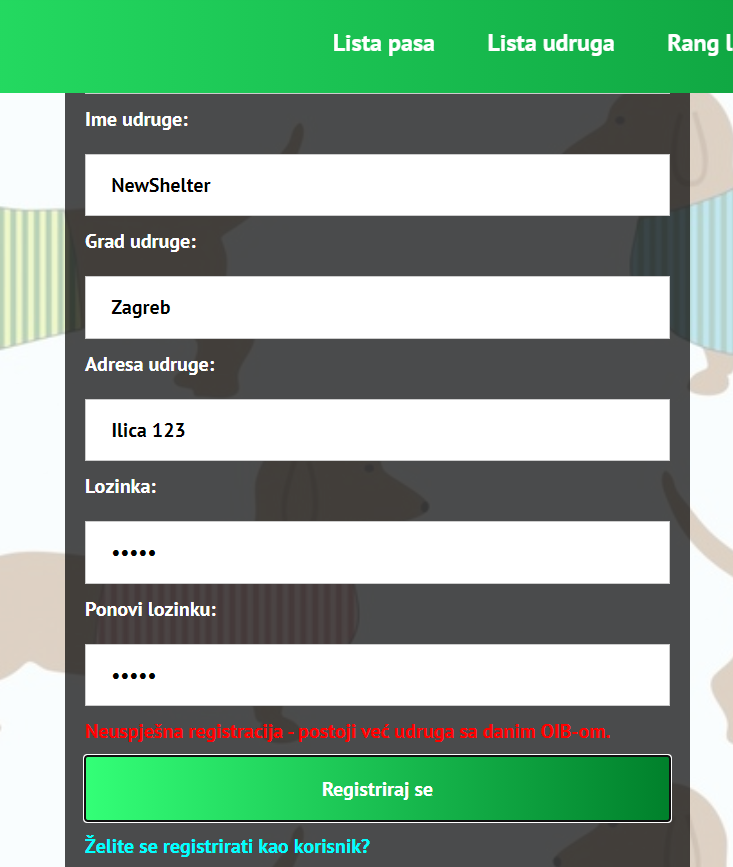
\includegraphics[scale=0.70]{slike/OIBError.PNG}
			 	%veličina slike u odnosu na originalnu datoteku i pozicija slike
			 	\centering
			 \end{figure}
			 \begin{figure}[H]
			 	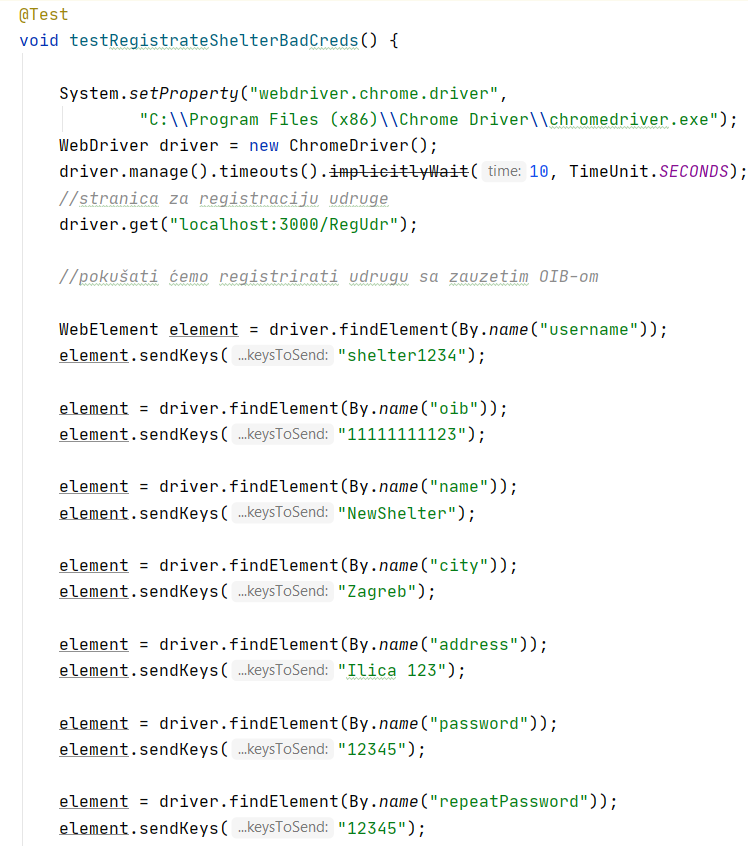
\includegraphics[scale=0.75]{slike/Selenium4.1.PNG}
			 	\hspace*{0.1in}
			 	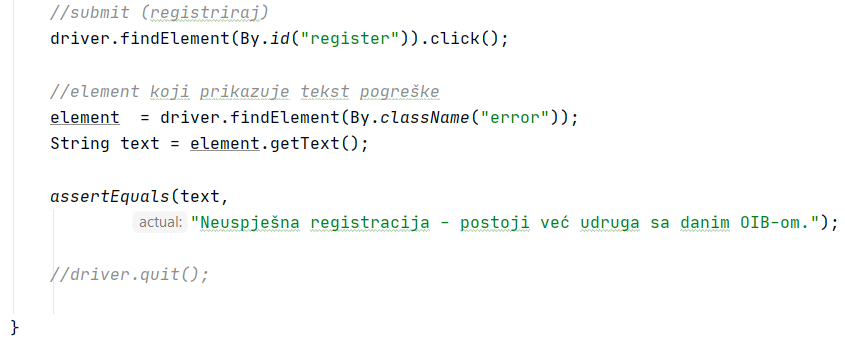
\includegraphics[scale=0.75]{slike/Selenium4.2.PNG} %veličina slike u odnosu na originalnu datoteku i pozicija slike
			 	\centering
			 \end{figure}
		 
		 
		 	\begin{figure}[H]
		 		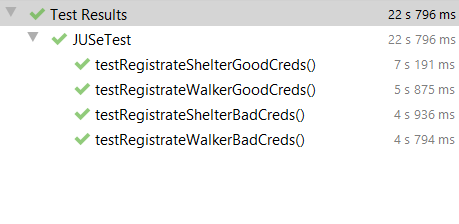
\includegraphics[scale=0.75]{slike/SeleniumRezultati.PNG} %veličina slike u odnosu na originalnu datoteku i pozicija slike
		 		\centering
		 	\end{figure}
		 
		 
			
			\eject 
		
		
		\section{Dijagram razmještaja}
			
			%\textbf{\textit{dio 2. revizije}}
			
			% \textit{Potrebno je umetnuti \textbf{specifikacijski} dijagram razmještaja i opisati ga. Moguće je umjesto specifikacijskog dijagrama razmještaja umetnuti dijagram razmještaja instanci, pod uvjetom da taj dijagram bolje opisuje neki važniji dio sustava.}
			
			\text Topologija našeg projekta sastoji se od dva čvora, od kojih su oba uređaji. Jedan je korisničko računalo, drugi je poslužiteljsko računalo. Na poslužiteljskom računalu nalaze se svi potrebni izvorni kodovi i baza podataka kako bi se ostvario uspješan deploy web aplikacije. Programska potpora sastoji se od kombinacije Spring frameworka i ReactJs-a. Također, korisničko i poslužiteljsko računalo međusobno razmjenjuju informacije putem HTTP protokola.
			
			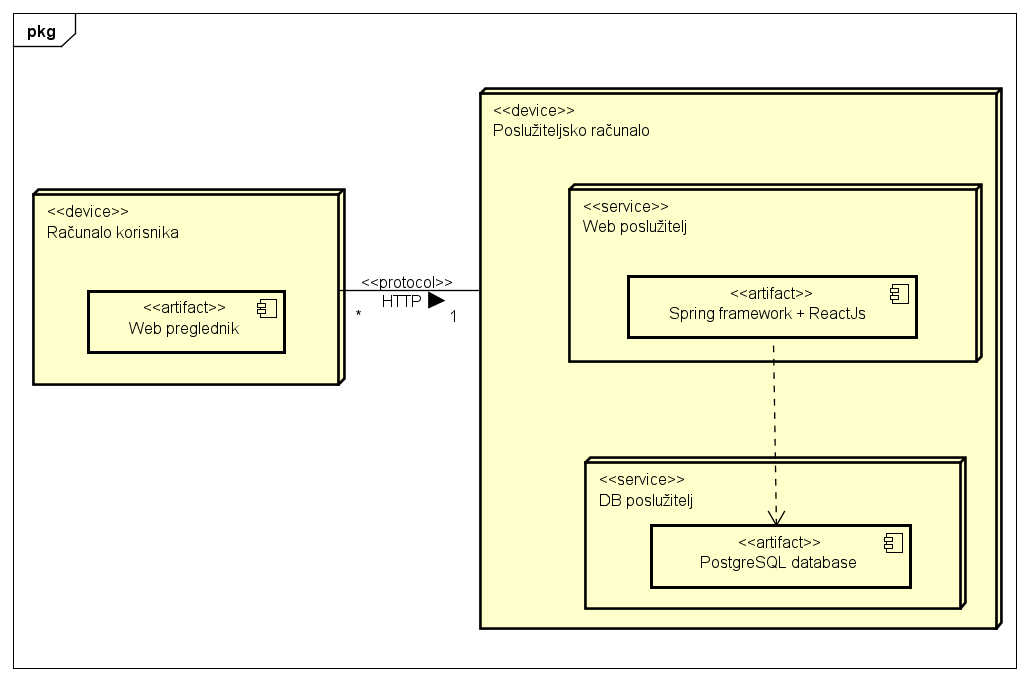
\includegraphics[scale=0.5]{dijagrami/Dijagram razmjestaja.png}
			
			\eject 
		
		\section{Upute za puštanje u pogon}
		
			\textbf{\textit{dio 2. revizije}}\\
		
			 \textit{U ovom poglavlju potrebno je dati upute za puštanje u pogon (engl. deployment) ostvarene aplikacije. Na primjer, za web aplikacije, opisati postupak kojim se od izvornog kôda dolazi do potpuno postavljene baze podataka i poslužitelja koji odgovara na upite korisnika. Za mobilnu aplikaciju, postupak kojim se aplikacija izgradi, te postavi na neku od trgovina. Za stolnu (engl. desktop) aplikaciju, postupak kojim se aplikacija instalira na računalo. Ukoliko mobilne i stolne aplikacije komuniciraju s poslužiteljem i/ili bazom podataka, opisati i postupak njihovog postavljanja. Pri izradi uputa preporučuje se \textbf{naglasiti korake instalacije uporabom natuknica} te koristiti što je više moguće \textbf{slike ekrana} (engl. screenshots) kako bi upute bile jasne i jednostavne za slijediti.}
			
			
			 \textit{Dovršenu aplikaciju potrebno je pokrenuti na javno dostupnom poslužitelju. Studentima se preporuča korištenje neke od sljedećih besplatnih usluga: \href{https://aws.amazon.com/}{Amazon AWS}, \href{https://azure.microsoft.com/en-us/}{Microsoft Azure} ili \href{https://www.heroku.com/}{Heroku}. Mobilne aplikacije trebaju biti objavljene na F-Droid, Google Play ili Amazon App trgovini.}
			
			
			\eject 
	\chapter{Zaključak i budući rad}
		
		\textbf{\textit{dio 2. revizije}}\\
		
		 \textit{U ovom poglavlju potrebno je napisati osvrt na vrijeme izrade projektnog zadatka, koji su tehnički izazovi prepoznati, jesu li riješeni ili kako bi mogli biti riješeni, koja su znanja stečena pri izradi projekta, koja bi znanja bila posebno potrebna za brže i kvalitetnije ostvarenje projekta i koje bi bile perspektive za nastavak rada u projektnoj grupi.}
		
		 \textit{Potrebno je točno popisati funkcionalnosti koje nisu implementirane u ostvarenoj aplikaciji.}
		
		\eject 
	\chapter*{Popis literature}
		\addcontentsline{toc}{chapter}{Popis literature}
	 	
 		\textbf{\textit{Kontinuirano osvježavanje}}
	
		\textit{Popisati sve reference i literaturu koja je pomogla pri ostvarivanju projekta.}
		
		
		\begin{enumerate}
			
			
			\item  Programsko inženjerstvo, FER ZEMRIS, \url{http://www.fer.hr/predmet/proinz}
			
			\item  I. Sommerville, "Software engineering", 8th ed, Addison Wesley, 2007.
			
			\item  T.C.Lethbridge, R.Langaniere, "Object-Oriented Software Engineering", 2nd ed. McGraw-Hill, 2005.
			
			\item  I. Marsic, Software engineering book``, Department of Electrical and Computer Engineering, Rutgers University, \url{http://www.ece.rutgers.edu/~marsic/books/SE}
			
			\item  The Unified Modeling Language, \url{https://www.uml-diagrams.org/}
			
			\item  Astah Community, \url{http://astah.net/editions/uml-new}
		\end{enumerate}
		
		 
	
	
	\begingroup
	\renewcommand*\listfigurename{Indeks slika i dijagrama}
	%\renewcommand*\listtablename{Indeks tablica}
	%\let\clearpage\relax
	\listoffigures
	%\vspace{10mm}
	%\listoftables
	\endgroup
	\addcontentsline{toc}{chapter}{Indeks slika i dijagrama}


	
	\eject 
		
	\chapter*{Dodatak: Prikaz aktivnosti grupe}
		\addcontentsline{toc}{chapter}{Dodatak: Prikaz aktivnosti grupe}
		
		\section*{Dnevnik sastajanja}
		
		
		\begin{packed_enum}
			\item  sastanak
			
			\item[] \begin{packed_item}
				\item Datum: 15. listopada 2020.
				\item Prisustvovali: L.Bokarica, A.Lukač, V. Sabalić, S. Almer, D. Lisica
				\item Teme sastanka:
				\begin{packed_item}
					\item specificiranje tehnologija za aplikaciju
					\item   specificiranje funkcionalnosti i zahtjeva aplikacije
					\item  entiteti baze podataka
				\end{packed_item}
			\end{packed_item}
			
			\item  sastanak
			\item[] \begin{packed_item}
				\item Datum: 22. listopada 2020.
				\item Prisustvovali: L.Bokarica, V. Sabalić, D. Lisica, P. Presečki
				\item Teme sastanka:
				\begin{packed_item}
					\item  pisanje backenda
					\item  rasprava o entitetima baze
				\end{packed_item}
			\end{packed_item}
		
			\item  sastanak
			\item[] \begin{packed_item}
				\item Datum: 29. listopada 2020.
				\item Prisustvovali: L.Bokarica, V. Sabalić, S. Almer, D. Lisica, J. Juroš, P. Presečki, A. Lukač
				\item Teme sastanka:
				\begin{packed_item}
					\item  pisanje backenda
					\item pisanje frontenda
					\item  sastanak sa asistenticom i usmjeravanje oko baze podataka
					\item dogovor oko pisanja dokumentacije
				\end{packed_item}
			\end{packed_item}
		
				\item  sastanak
			\item[] \begin{packed_item}
				\item Datum: 7. studenoga 2020.
				\item Prisustvovali: L.Bokarica, V. Sabalić, S. Almer, D. Lisica, J. Juroš, P. Presečki, A. Lukač
				\item Teme sastanka:
				\begin{packed_item}
					\item  pisanje backenda
					\item pisanje frontenda
					\item osposobljavanje login-a i signup-a korisnika
					\item  dogovor oko pisanja dokumentacije
				\end{packed_item}
			\end{packed_item}
		
				\item  sastanak
			\item[] \begin{packed_item}
				\item Datum: 12. prosinca 2020.
				\item Prisustvovali: L.Bokarica, V. Sabalić, S. Almer, D. Lisica, J. Juroš, P. Presečki, A. Lukač
				\item Teme sastanka:
				\begin{packed_item}
					\item  pisanje backenda
					\item pisanje frontenda
					\item dodavanje novih funkcionalnosti na frontendu i backendu:
					\begin{packed_item}
						\item dodavanje autorizacija
						\item slanje zahtjeva s frontenda
						\item stranice profila pasa, šetača, udruga
					\end{packed_item}	
				\end{packed_item}
			\end{packed_item}
				\item sastanak
				\item[] \begin{packed_item}
				\item Datum: 4. siječnja 2021.
				\item Prisustvovali: L.Bokarica, V. Sabalić, S. Almer, D. Lisica, J. Juroš, P. Presečki, A. Lukač
				\item Teme sastanka:
				\begin{packed_item}
					\item  pisanje backenda
					\item pisanje frontenda
					\item dodavanje novih funkcionalnosti na frontendu i backendu:
					\begin{packed_item}
						\item dodavanje pasa
						\item uređivanje pasa
						\item rezervacija šetnji
						\item prikaz statistika šetnji
					\end{packed_item}	
				\end{packed_item}
			\end{packed_item}
			
			%
			
		\end{packed_enum}
		
		\eject
		\section*{Tablica aktivnosti}					
			
			\begin{longtabu} to \textwidth {|X[7, l]|X[1, c]|X[1, c]|X[1, c]|X[1, c]|X[1, c]|X[1, c]|X[1, c]|}
								
				\cline{2-8} \multicolumn{1}{c|}{\textbf{}} &     \multicolumn{1}{c|}{\rotatebox{90}{\textbf{Jana Juroš }}} & \multicolumn{1}{c|}{\rotatebox{90}{\textbf{Anamarija Lukač }}} &	\multicolumn{1}{c|}{\rotatebox{90}{\textbf{Petra Presečki }}} &	\multicolumn{1}{c|}{\rotatebox{90}{\textbf{Luka Bokarica }}} &
				\multicolumn{1}{c|}{\rotatebox{90}{\textbf{David Lisica }}} &
				\multicolumn{1}{c|}{\rotatebox{90}{\textbf{Vito Sabalić }}} &	\multicolumn{1}{c|}{\rotatebox{90}{\textbf{Sven Almer }}} \\ \hline 
				\endfirsthead
				
			
				\cline{2-8} \multicolumn{1}{c|}{\textbf{}} &     \multicolumn{1}{c|}{\rotatebox{90}{\textbf{Jana Juroš}}} & \multicolumn{1}{c|}{\rotatebox{90}{\textbf{Anamarija Lukač }}} &	\multicolumn{1}{c|}{\rotatebox{90}{\textbf{Petra Presečki }}} &
				\multicolumn{1}{c|}{\rotatebox{90}{\textbf{Luka Bokarica }}} &	\multicolumn{1}{c|}{\rotatebox{90}{\textbf{David Lisica }}} &
				\multicolumn{1}{c|}{\rotatebox{90}{\textbf{Vito Sabalić }}} &	\multicolumn{1}{c|}{\rotatebox{90}{\textbf{Sven Almer }}} \\ \hline 
				\endhead
				
				
				\endfoot
							
				 
				\endlastfoot
				

				Upravljanje projektom 		& 6 & 2 & 0 & 3 & 2 & 1 & 1\\ \hline
				Opis projektnog zadatka 	& 3 & 3 & 0 & 2 & 2 & 0 & 1\\ \hline
				
				Funkcionalni zahtjevi       & 1.5 & 3 & 0 & 1 & 1.5 & 0 & 1 \\ \hline
				Opis pojedinih obrazaca 	& 3 & 4 &0  & 0.5 & 2.5 & 0.5 & 0 \\ \hline
				Dijagram obrazaca 			&1.5 & 1 & 0 & 0 & 1 & 0 & 0 \\ \hline
				Sekvencijski dijagrami 		& 3 & 1 & 0 & 0 & 0.5 & 0.5 & 0 \\ \hline
				Opis ostalih zahtjeva 		& 0.5 & 0 & 0 & 0 & 1 & 0 & 0 \\ \hline

				Arhitektura i dizajn sustava	 & 2.5 & 4 & 0 & 4 & 2 & 0 & 3 \\ \hline
				Baza podataka				& 0.5  & 7 & 0 & 8 & 7 & 0 & 4 \\ \hline
				Dijagram razreda 			& 0 & 1 & 0 & 1 & 1 & 0 & 0.5 \\ \hline
				Dijagram stanja				& 0 & 0 &0  & 0 & 0 & 0 & 0 \\ \hline
				Dijagram aktivnosti 		& 0 & 0 & 0 & 0 & 0 & 0 & 0.5 \\ \hline
				Dijagram komponenti			& 0 & 0 & 0 & 0 & 0 & 0 & 0 \\ \hline
				Korištene tehnologije i alati 		& 0 & 0 &0  & 0 & 0 & 0 & 0 \\ \hline
				Ispitivanje programskog rješenja 	& 12 & 0 &0  & 0 & 0 & 0 & 0 \\ \hline
				Dijagram razmještaja			&0  & 0 &0  & 0 & 0 & 0 & 0 \\ \hline
				Upute za puštanje u pogon 		& 0 & 0 &0  & 0 & 0 & 0 & 0 \\ \hline
				Dnevnik sastajanja 			& 0.5 & 0 & 0 & 0.5 & 1 & 0 & 0 \\ \hline
				Zaključak i budući rad 		& 0.5 & 0 & 0 & 0 & 0 & 0 & 0 \\  \hline
				Popis literature 			& 0.5 & 0 &0  & 0 & 0 & 0 & 0 \\  \hline
				&  &  &  &  &  &  &  \\ \hline \hline
		
				front end				& 30 & 1 & 14 & 1 & 1 & 14 & 0 \\ \hline 
				 izrada baze podataka 	& 0 & 3 & 0 & 5 & 5 & 2 & 4\\ \hline 
				spajanje s bazom podataka 	& 0 & 2 & 0 & 0.5 & 0 & 0 & 0 \\ \hline
				back end							& 4 & 25 & 0 & 40 & 30 & 0 & 15 \\  \hline
				 							&  &  &  &  &  &  &\\  \hline
				
				
			\end{longtabu}
					
					
		\eject
		\section*{Dijagrami pregleda promjena}
		
		\begin{figure}[H]
			\hspace*{-0.54in}
			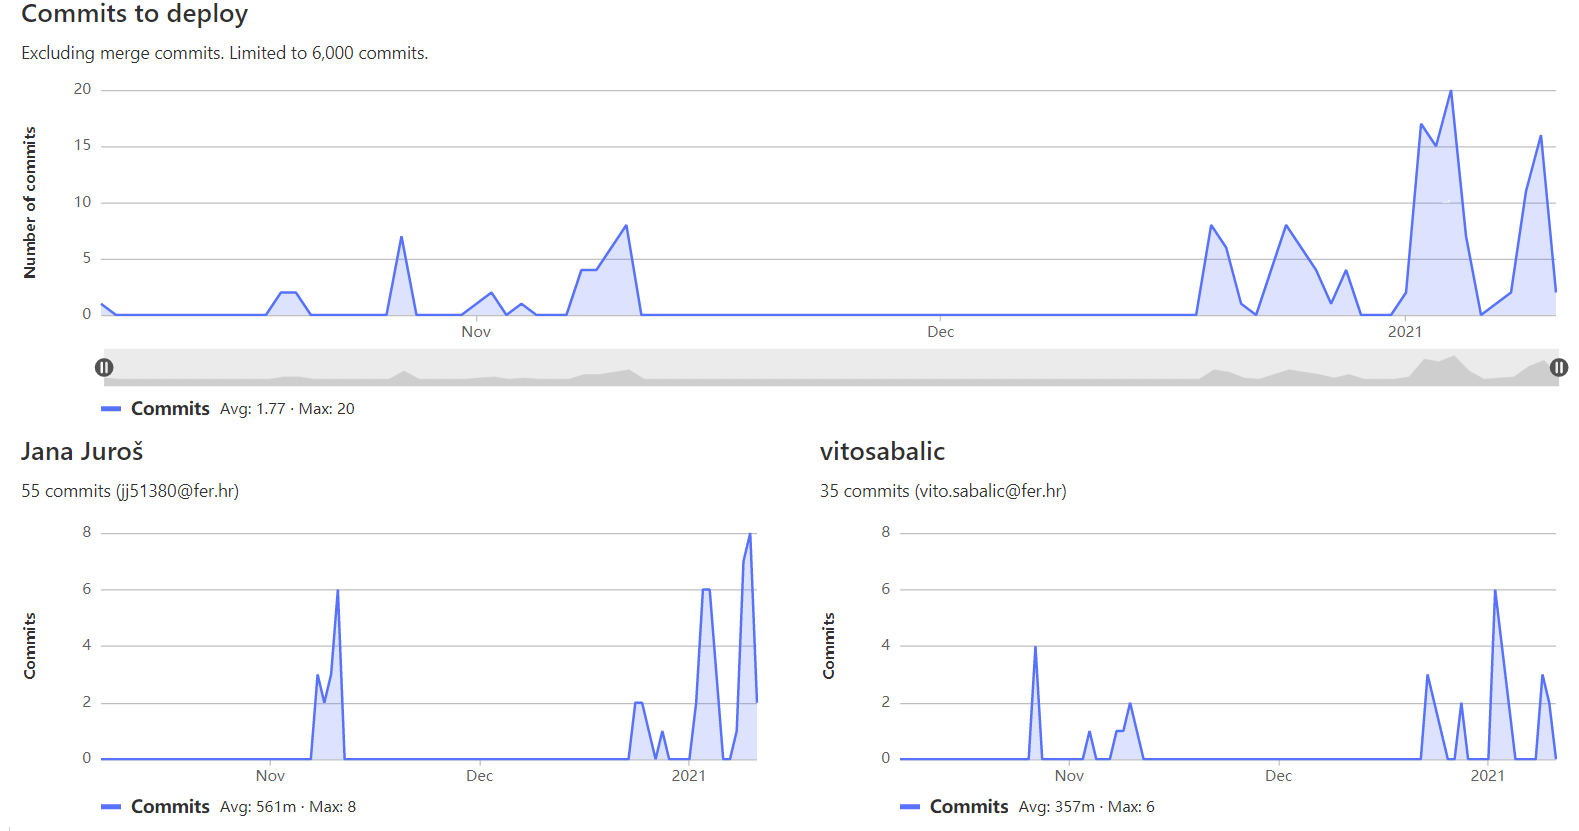
\includegraphics[scale=0.43]{dijagrami/Dijagram pregleda promjena1.png}
			%veličina slike u odnosu na originalnu datoteku i pozicija slike
			\label{fig:Dijagram pregleda promjena 1}
			\centering
		\end{figure}
	
		\begin{figure}[H]
			\hspace*{-0.54in}
			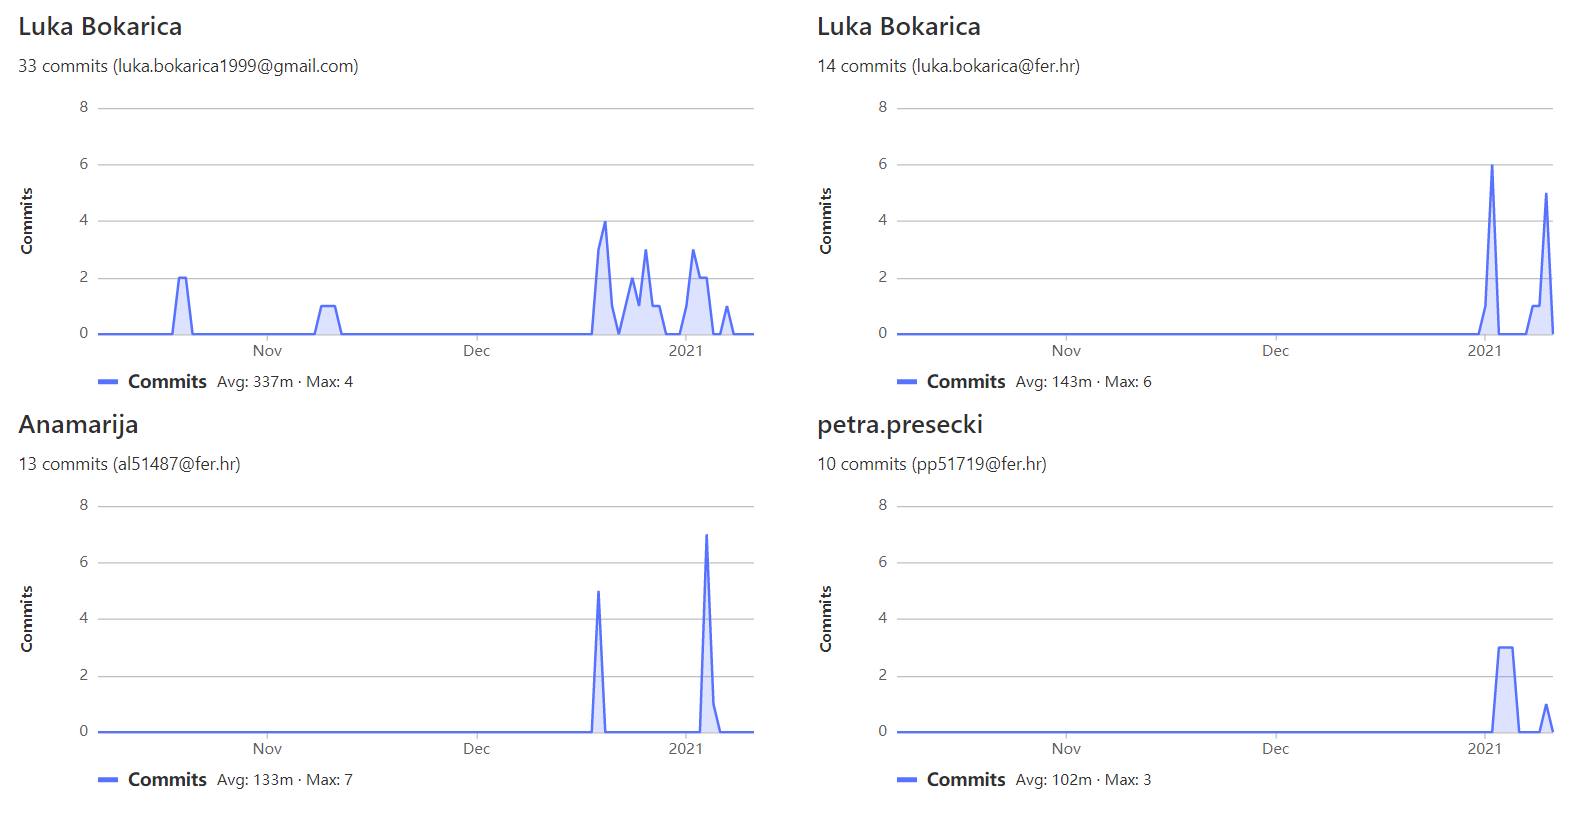
\includegraphics[scale=0.43]{dijagrami/Dijagram pregleda promjena2.1.png}
			%veličina slike u odnosu na originalnu datoteku i pozicija slike
			\label{fig:Dijagram pregleda promjena 2}
			\centering
		\end{figure}
		
		\begin{figure}[H]
			\hspace*{-0.54in}
			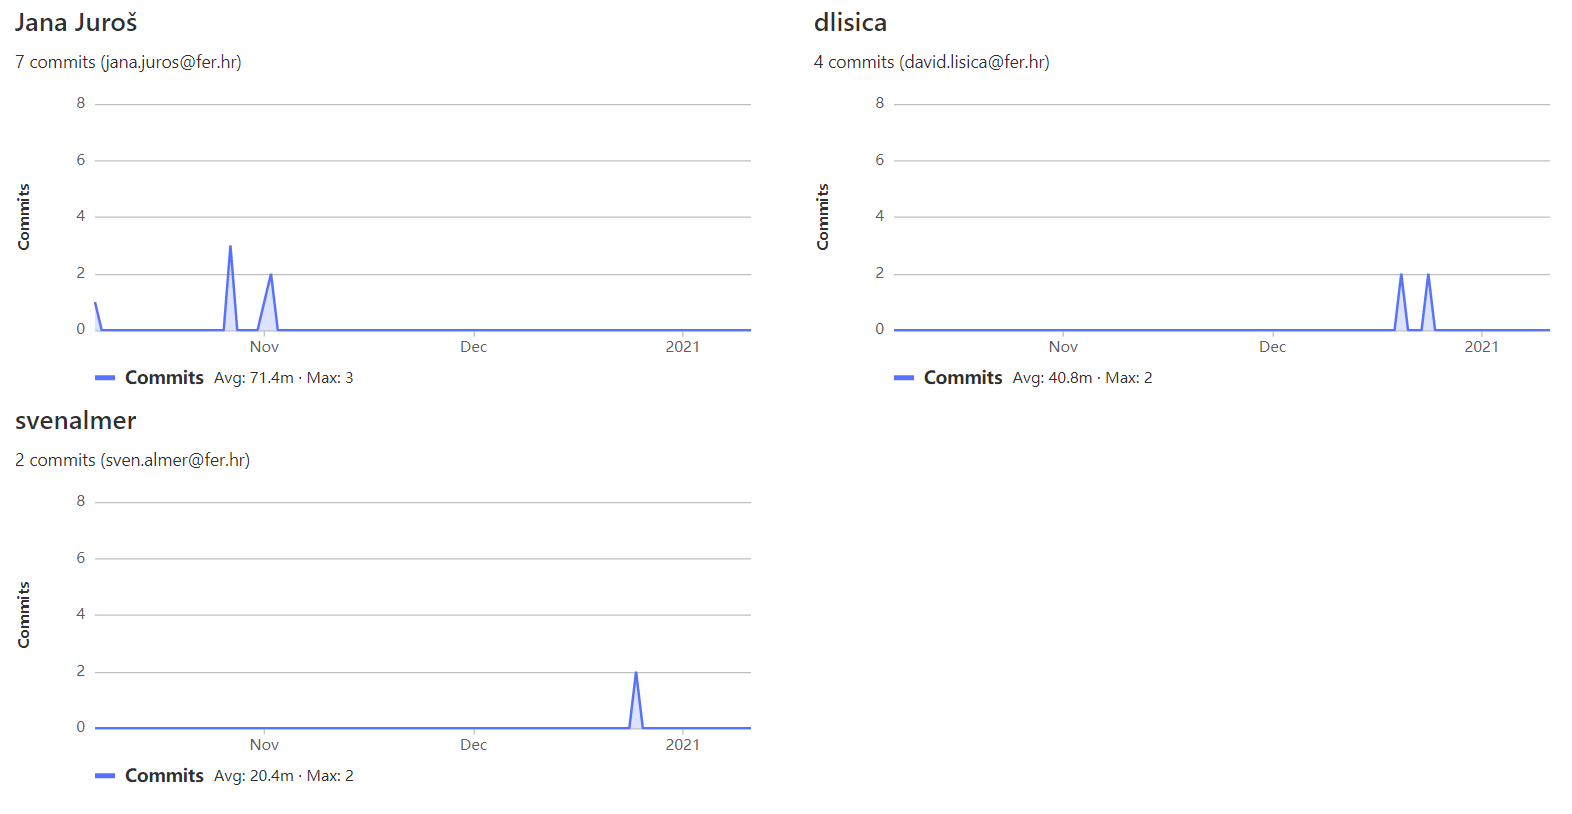
\includegraphics[scale=0.43]{dijagrami/Dijagram pregleda promjena2.png}
			\caption{Dijagrami pregleda promjena}
			%veličina slike u odnosu na originalnu datoteku i pozicija slike
			\label{fig:Dijagram pregleda promjena 3}
			\centering
		\end{figure}
		


\end{document} %naredbe i tekst nakon ove naredbe ne ulaze u izgrađen dokument 


